\documentclass[14pt, a4paper]{report}
\usepackage{mathtext}
\usepackage[T2A]{fontenc}
\usepackage[utf8]{inputenc}
\usepackage[russian]{babel}
\usepackage{multirow}
\usepackage{slashbox}
\usepackage{makecell}
\usepackage{graphicx}
\usepackage{physics}
\usepackage{amstext}
\usepackage{caption}
\usepackage{subcaption}
\usepackage{cmap}
\usepackage{float}
\usepackage{indentfirst}
\usepackage{romannum}
\usepackage{wasysym}

\usepackage[a4paper,
            		left=1in,
            		right=1in,
           		 top=1in,
            		bottom=1in,
            		footskip=.25in]{geometry}

\renewcommand{\thesection}{\arabic{section}.}
\renewcommand{\thesubsection}{\arabic{section}.\arabic{subsection}.}

\title{\textbf{Отчет о выполнении лабораторной работы 5.5. "Компьютерная сцинтилляционная $\gamma$ - спектрометрия"}}
\author{Калашников Михаил, Б03-202}
\date{}

\begin{document}
\maketitle

\pagenumbering{arabic}

\section{Теоретические сведения}

Основными процессами взаимодействия гамма-излучения с веществом являются, как было выше указано, фотоэффект, эффект Комптона и образование электрон-позитронных пар. Каждый из этих процессов вносит свой вклад в образование наблюдаемого спектра.

\textbf{Фотоэффект} -- процесс взаимодействия гамма-кванта с электроном, связанным с атомом, при котором электрону передается вся энергия гамма-кванта. При этом электрону сообщается кинетическая энергия $Т_e = Е_\gamma-I_i$, где $Е_\gamma$ -- энергия гамма-кванта, $I_i$ -- потенциал ионизации i-той оболочки атома. Фотоэффект особенно существенен для тяжелых веществ, где он идет с заметной вероятностью даже при высоких энергиях гамма-квантов. В легких веществах фотоэффект становится заметен лишь при относительно небольших энергиях гамма-квантов.

\textbf{Эффект Комптона} -- упругое рассеяние фотона на свободном электроне, сопровождающееся изменением длины волны фотона (реально этот процесс происходит на слабо связанных с атомом внешних электронах). Максимальная энергия образующихся комптоновских электронов соответствует рассеянию гамма-квантов на $180^\circ$ и равна

\[E_{max}=\frac{\hbar\omega}{1+\frac{mc^2}{2\hbar\omega}}\text{.}\]

\textbf{Процесс образования электрон-позитронных пар.} При достаточно высокой энергии гамма-кванта наряду с фотоэффектом и эффектом Комптона может происходить третий вид взаимодействия гамма-квантов с веществом -- образование электрон-позитронных пар. Процесс образования пар не может происходить в пустоте, так как в этом случае не выполняются совместно законы сохранения энергии и импульса. В присутствии ядра или электрона процесс образования пары гамма-квантом возможен, так как можно распределить энергию и импульс гамма-кванта между тремя частицами без противоречия с законами сохранения. При этом если процесс образования пары идет в кулоновском поле ядра, то энергия образующегося ядра отдачи оказывается весьма малой, так что пороговая энергия гамма-кванта $E_{пор}$, необходимая для образования пары, практически совпадает с удвоенной энергией покоя электрона $E_{пор}\approx 2mc^2 =1.022\ МэВ$.

\section{Экспериментальная установка}

\begin{figure}[H]
\centering
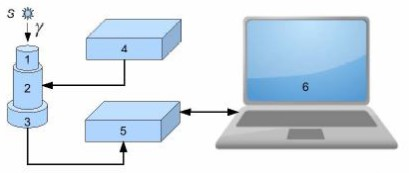
\includegraphics[width=.7\textwidth]{../images/555-1}
\caption{Принципиальная блок-схема спектрометра. (1 -- сцинтиллятор, 2 -- ФЭУ, 3 -- предусилитель импульсов, 4 -- высоковольтный блок питания для ФЭУ, 5 -- блок преобразования аналоговых импульсов с ФЭУ в цифровой код (АЦП), 6 -- компьютер для сбора данных, их обработки и хранения).}
\end{figure}

ФЭУ со сцинтиллятором и блоком питания установлены на отдельной подставке. В нашей работе на разных установках (стендах) в качестве сцинтиллятора используются кристаллы NaI(Tl) с размерами $\diameter\ 45\times50\ мм$ и $\diameter\ 20\times25\ мм$.

\section{Проведение эксперимента}

Проведем последовательные измерения спектров каждого из предоставленных образцов. Будем накапливать измерения в течение 600 секунд. После этого аналогично проведем измерения фонового излучения.

\begin{figure}[H]
\centering
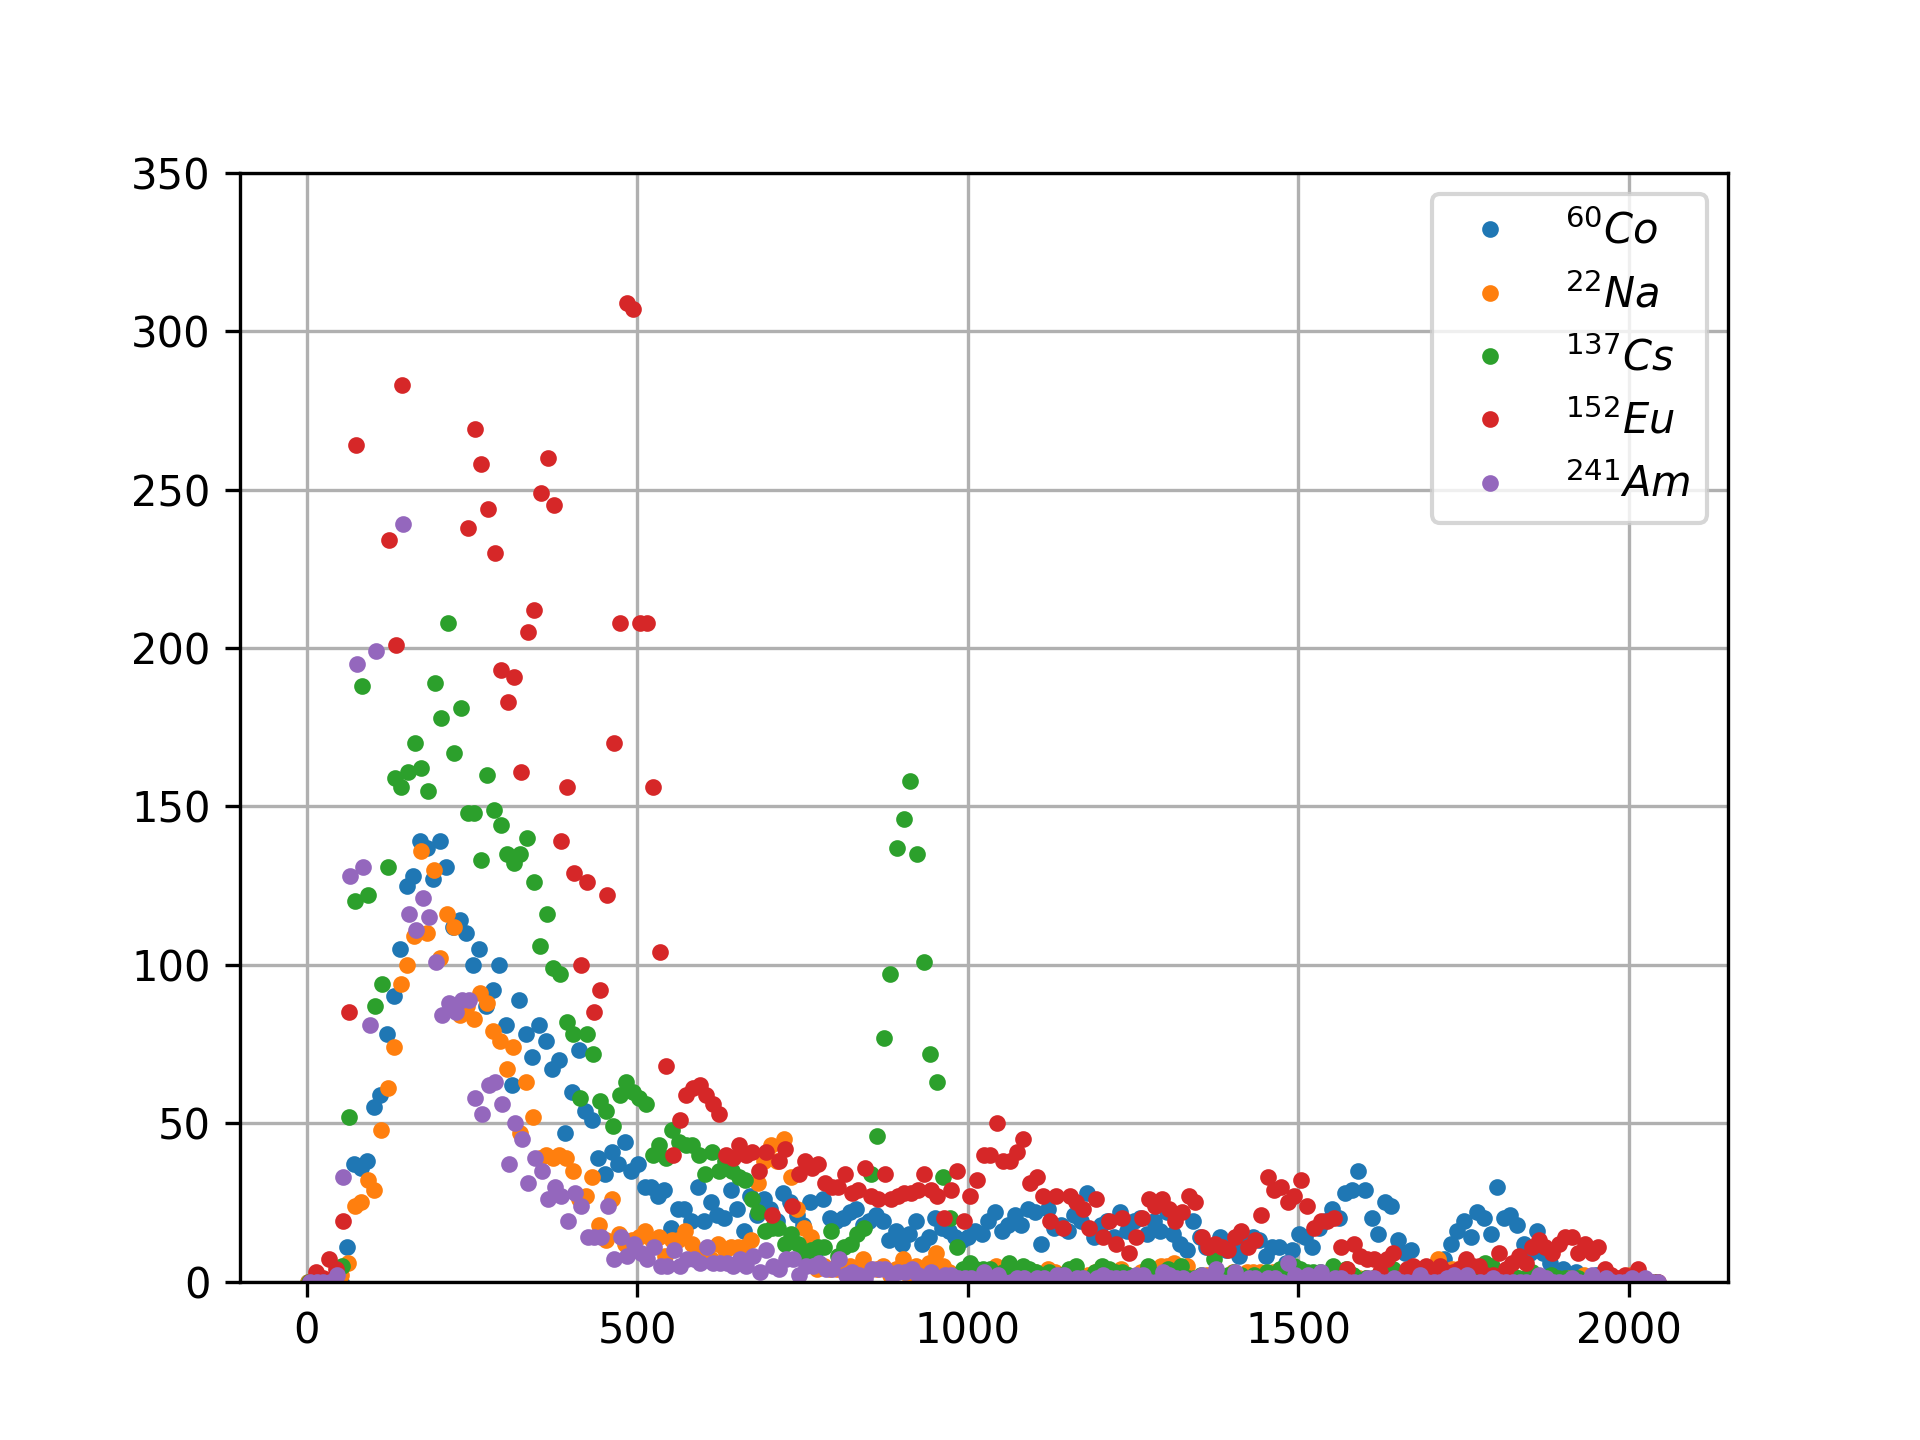
\includegraphics[width=.7\textwidth]{../images/555-common}
\caption{Спектр излучения образцов}
\end{figure}

Далее в работе будет приведено более подробное рассмотрение каждого из полученных спектров.

\begin{figure}[H]
\centering
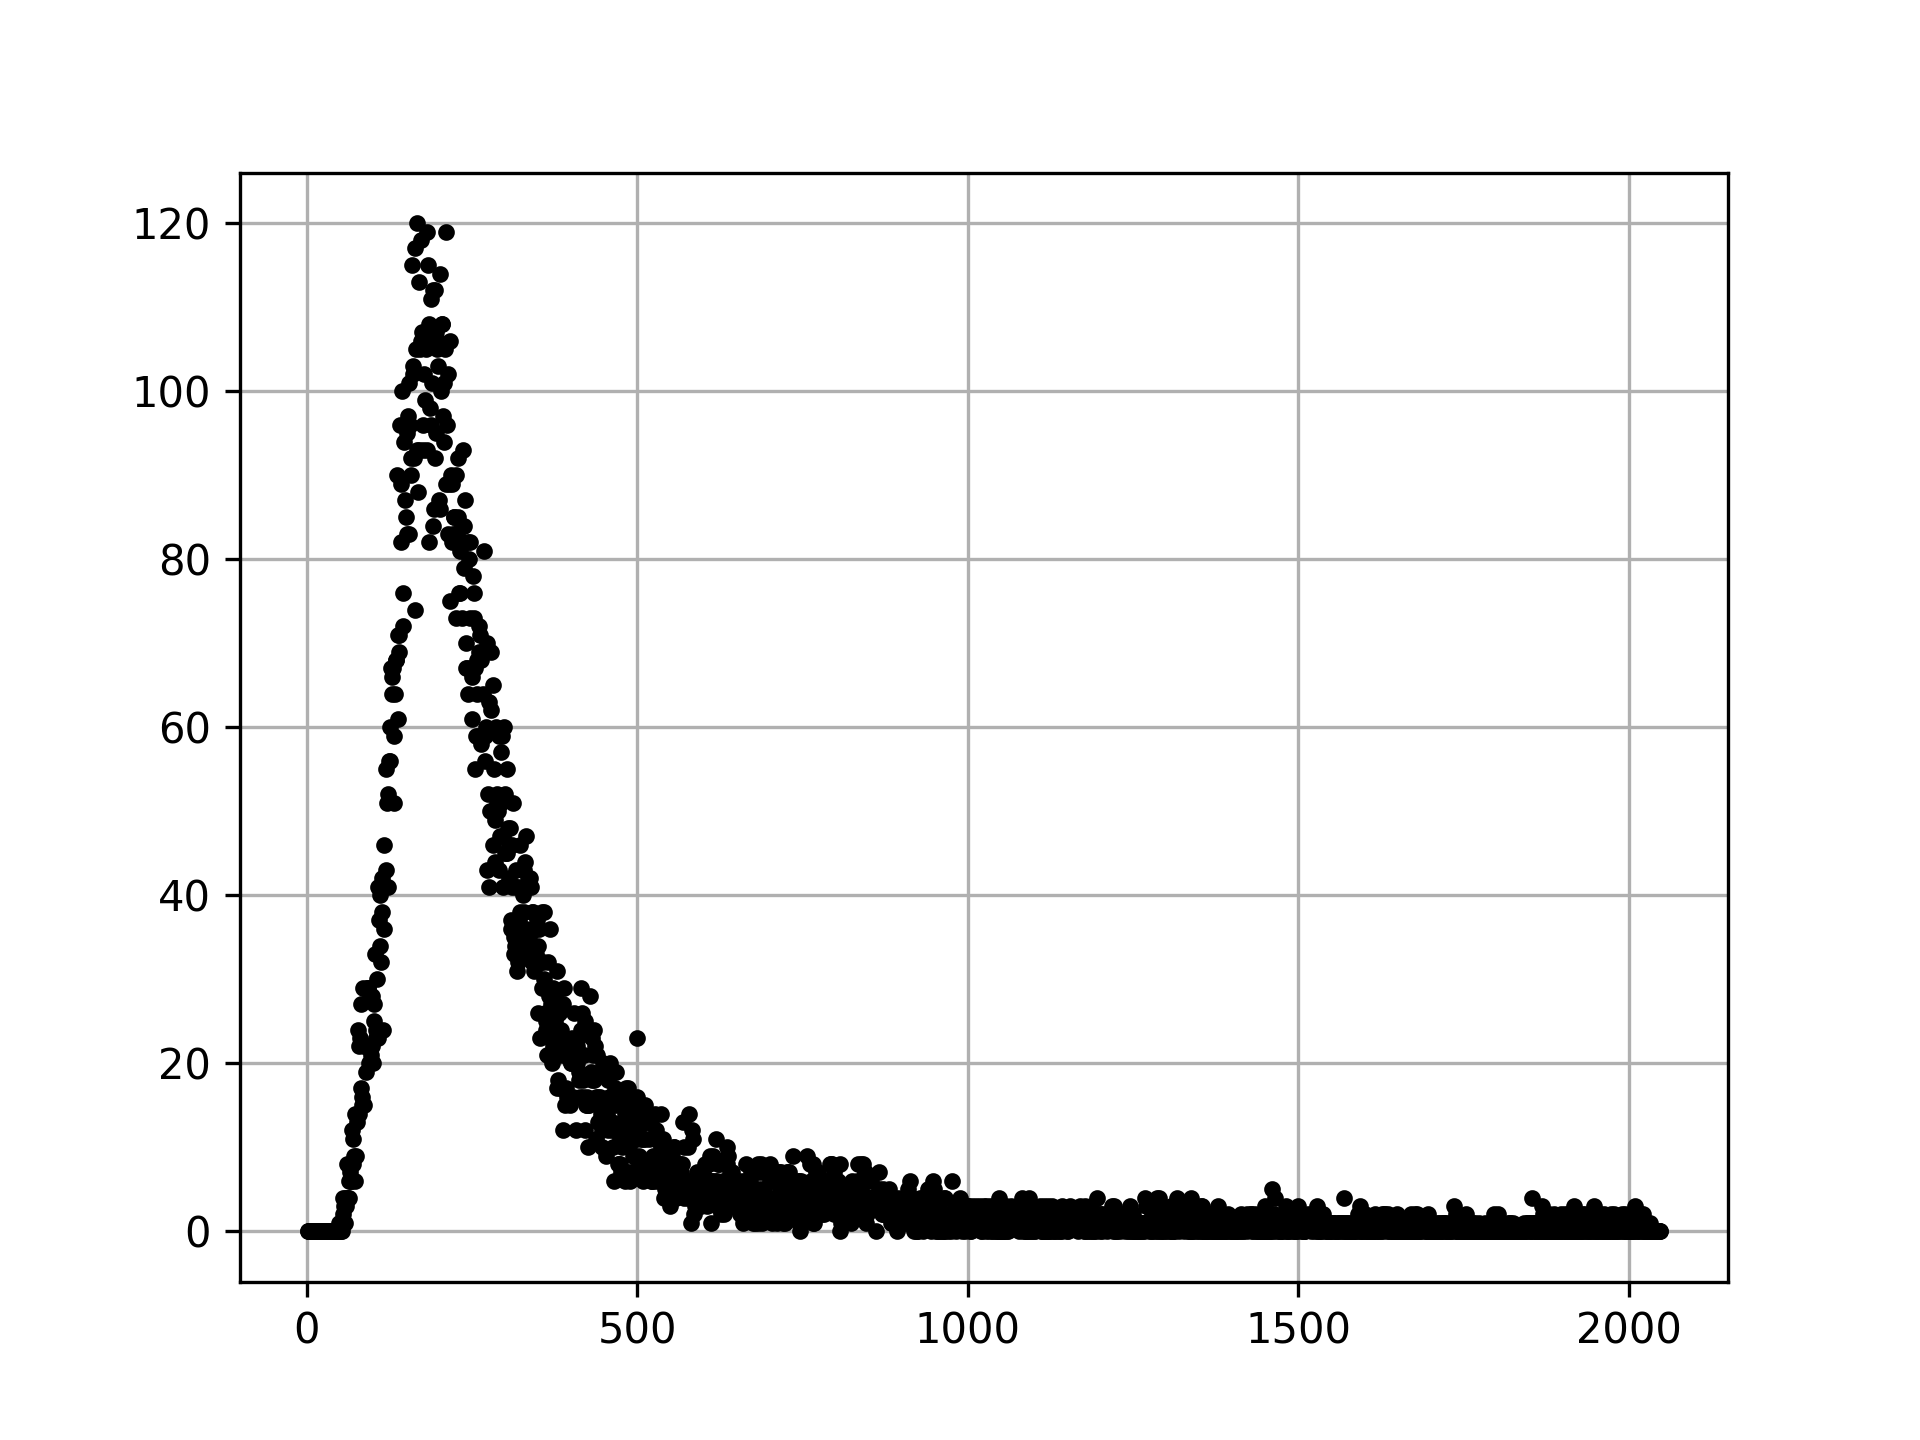
\includegraphics[width=.7\textwidth]{../images/555-bg}
\caption{Спектр фонового излучения}
\end{figure}

Как можно видеть, правая часть спектра фонового излучения является равномерной и не имеет резких скачков.

\section{Обработка результатов}

Приступим к определению положений фотопиков образцов.

\subsection{$^{60}\text{Co}$}

\begin{figure}[H]
\centering
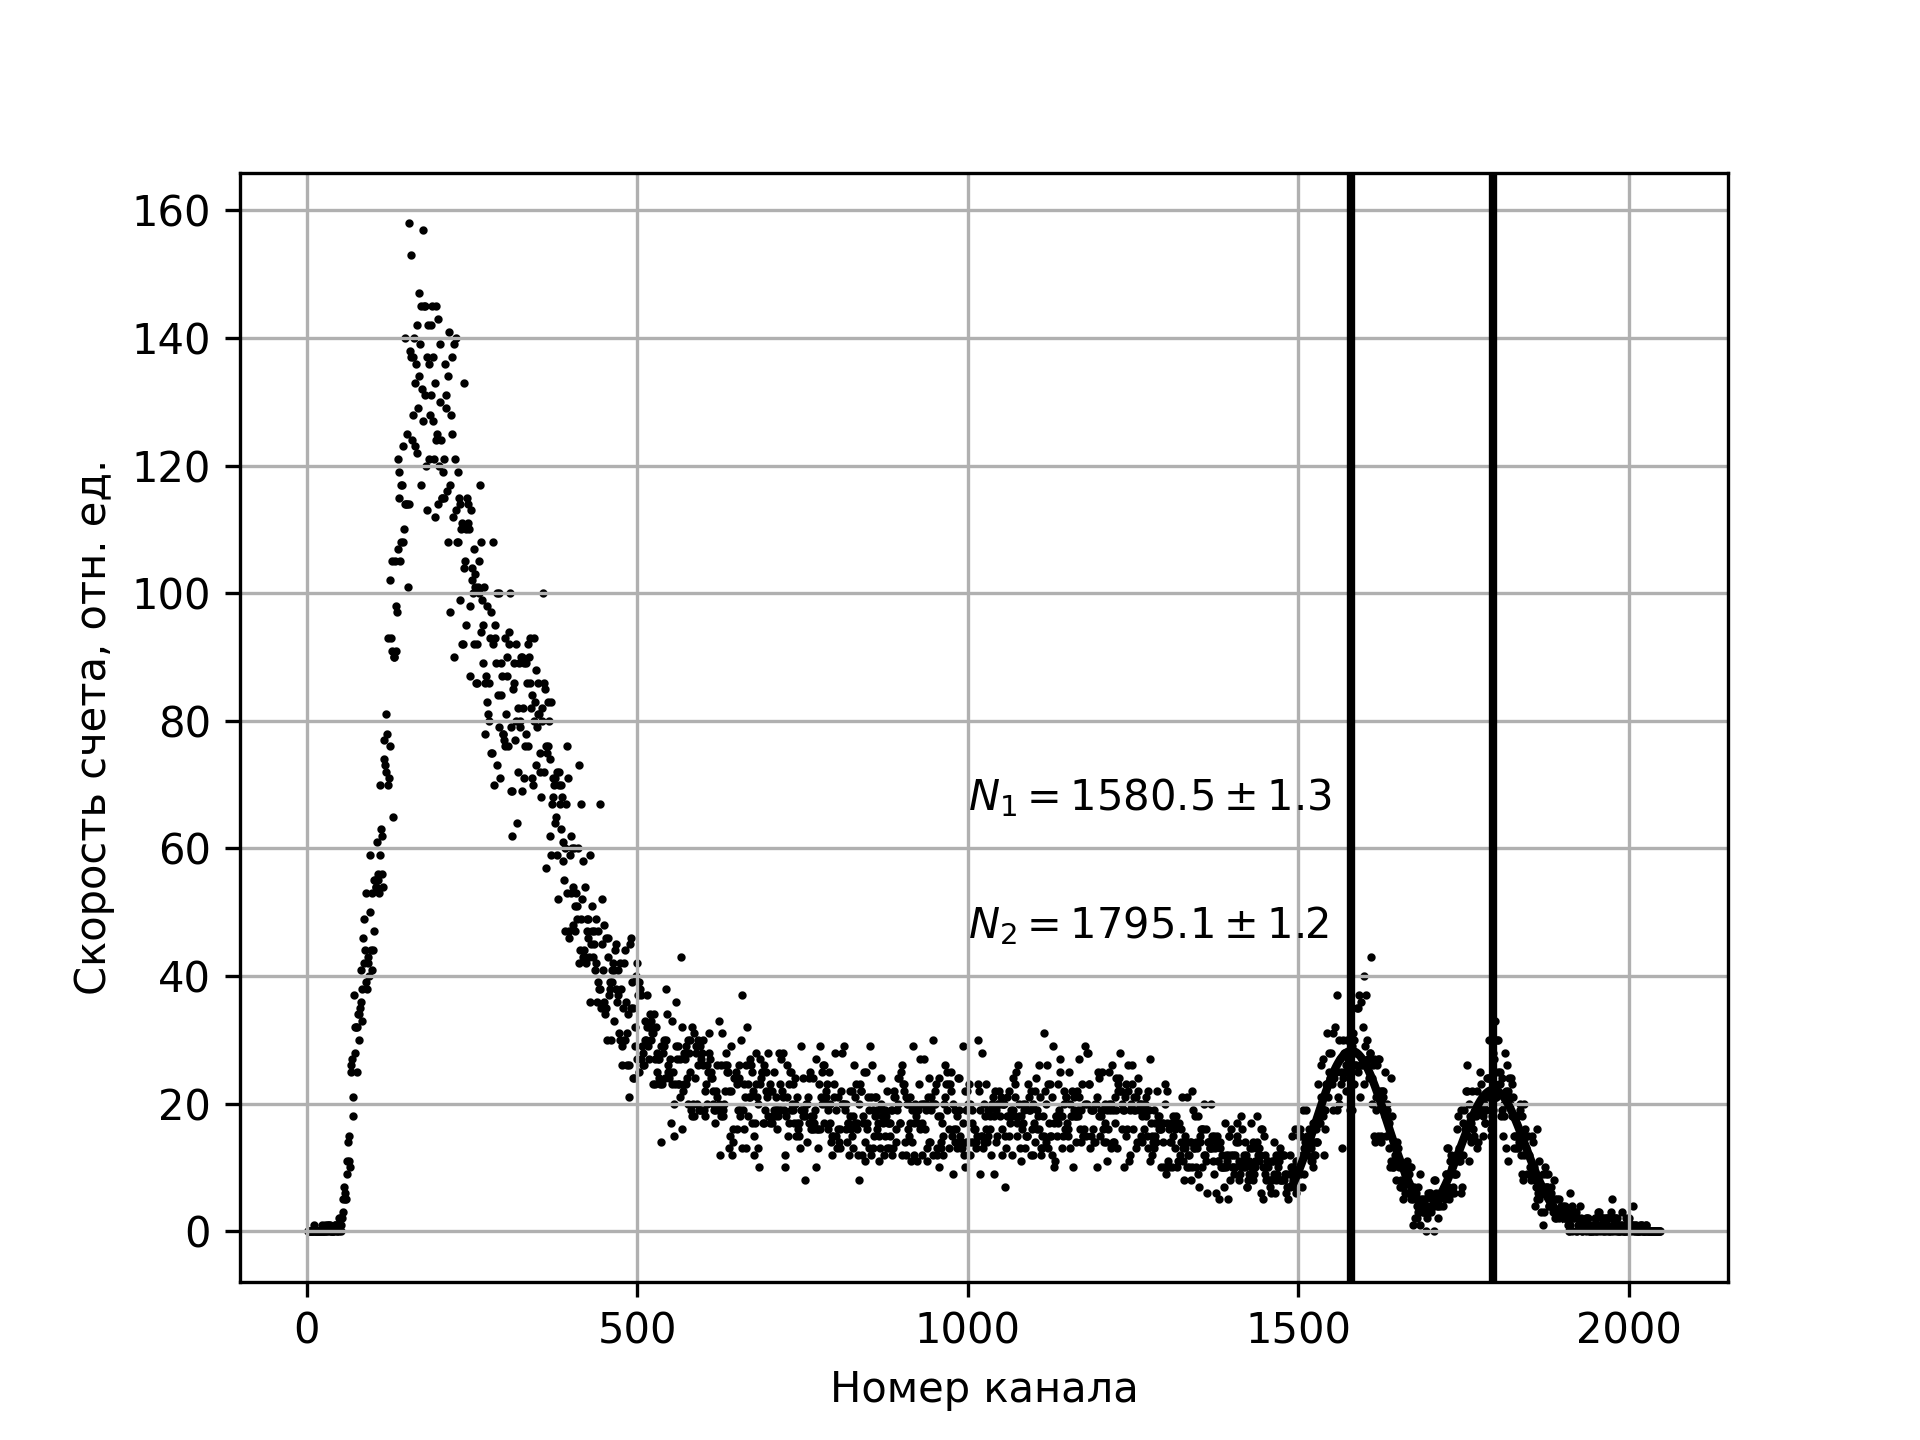
\includegraphics[width=.7\textwidth]{../images/555-co60}
\caption{Спектр излучения $^{60}\text{Co}$}
\end{figure}

В спектре кобальта-60 присутствуют два фотопика с энергиями $E_1=1.1732\ \text{МэВ}$ и $E_2=1.3325\ \text{МэВ}$.

\subsection{$^{22}\text{Na}$}

\begin{figure}[H]
\centering
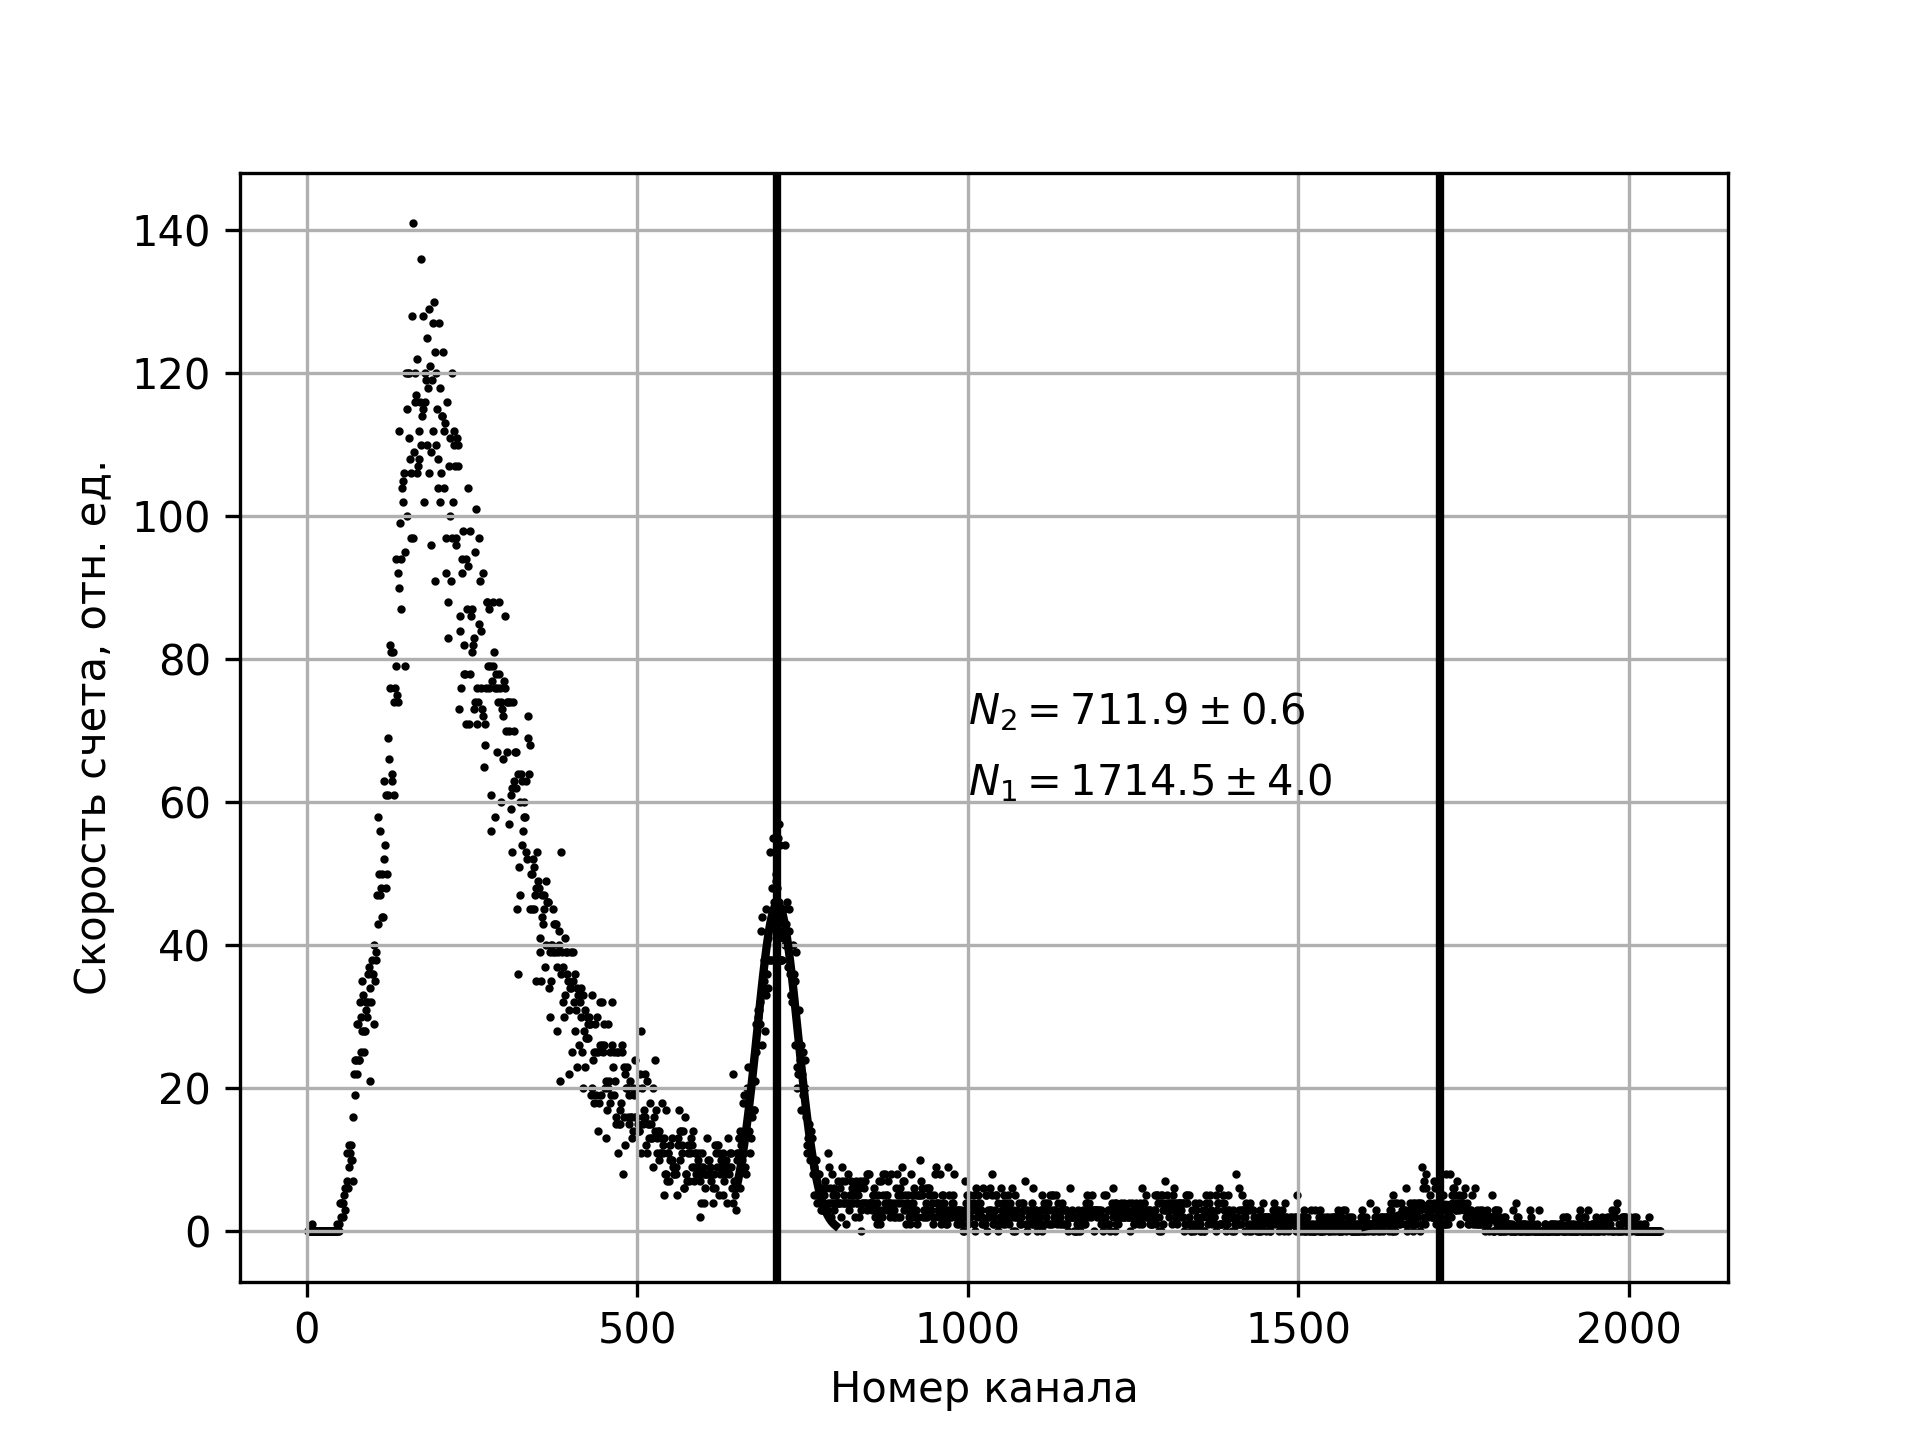
\includegraphics[width=.7\textwidth]{../images/555-na22}
\caption{Спектр излучения $^{22}\text{Na}$}
\end{figure}

В спектре натрия-22 присутствуют два фотопика с энергиями $E_1=1.274\ \text{МэВ}$ и $E_2=0.511\ \text{МэВ}$.

\subsection{$^{137}\text{Cs}$}

\begin{figure}[H]
\centering
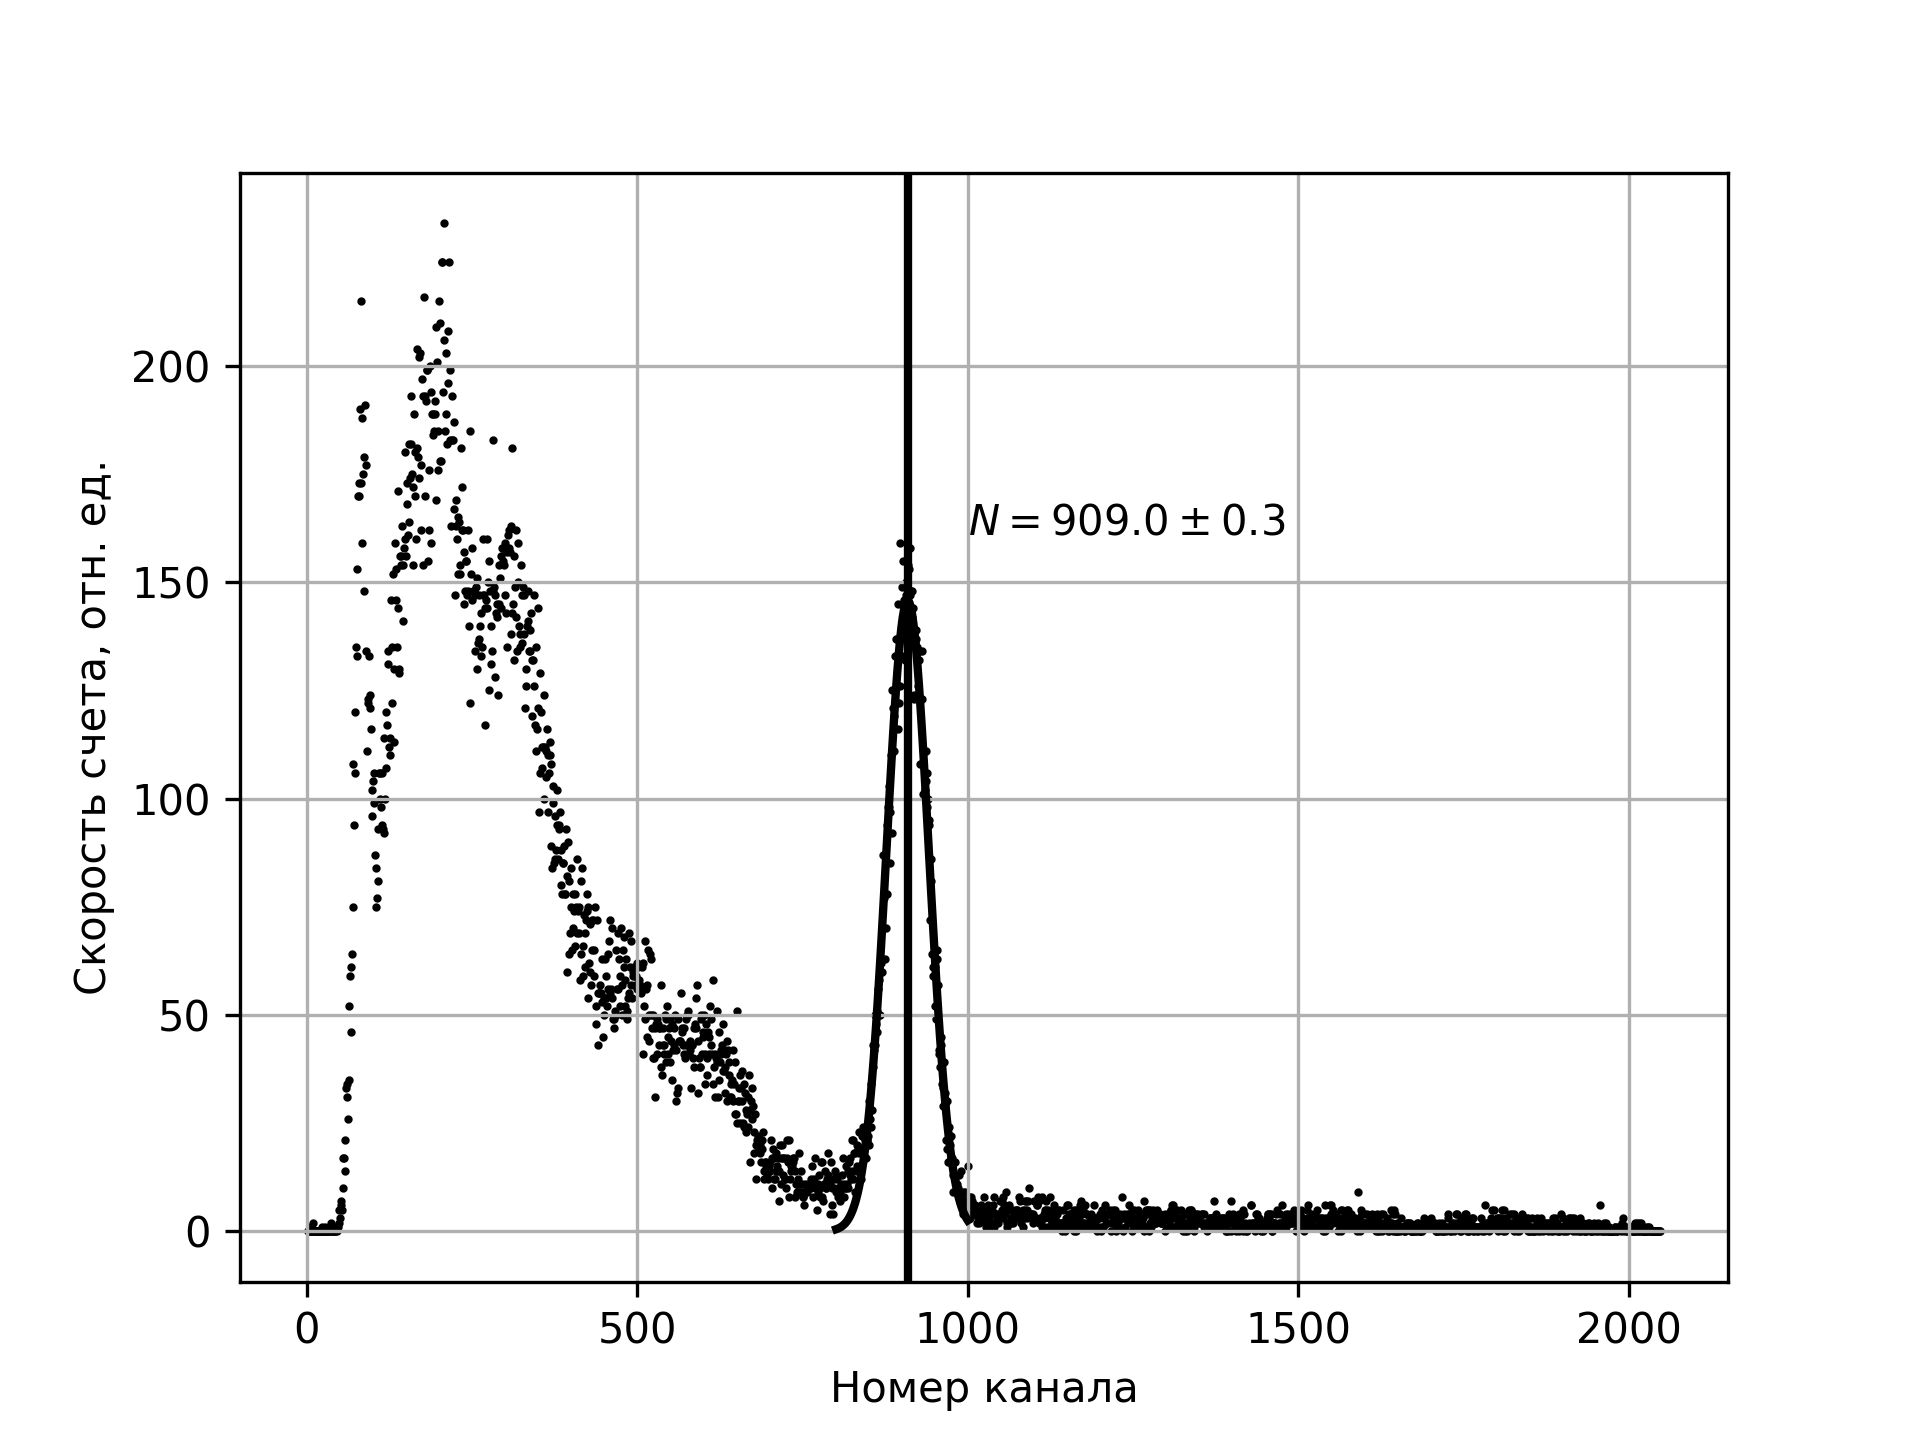
\includegraphics[width=.7\textwidth]{../images/555-cs137}
\caption{Спектр излучения $^{137}\text{Cs}$}
\end{figure}

В спектре цезия-137 присутствует фотопик с энергией $E=0.6617\ \text{МэВ}$.

\subsection{Калибровка}

После обработки всех элементов с известными положениями пиков проведем калибровку энергетической шкалы. Проведем прямую через полученные точки чтобы получить зависимость вида $N=aE+b$.

\begin{figure}[H]
\centering
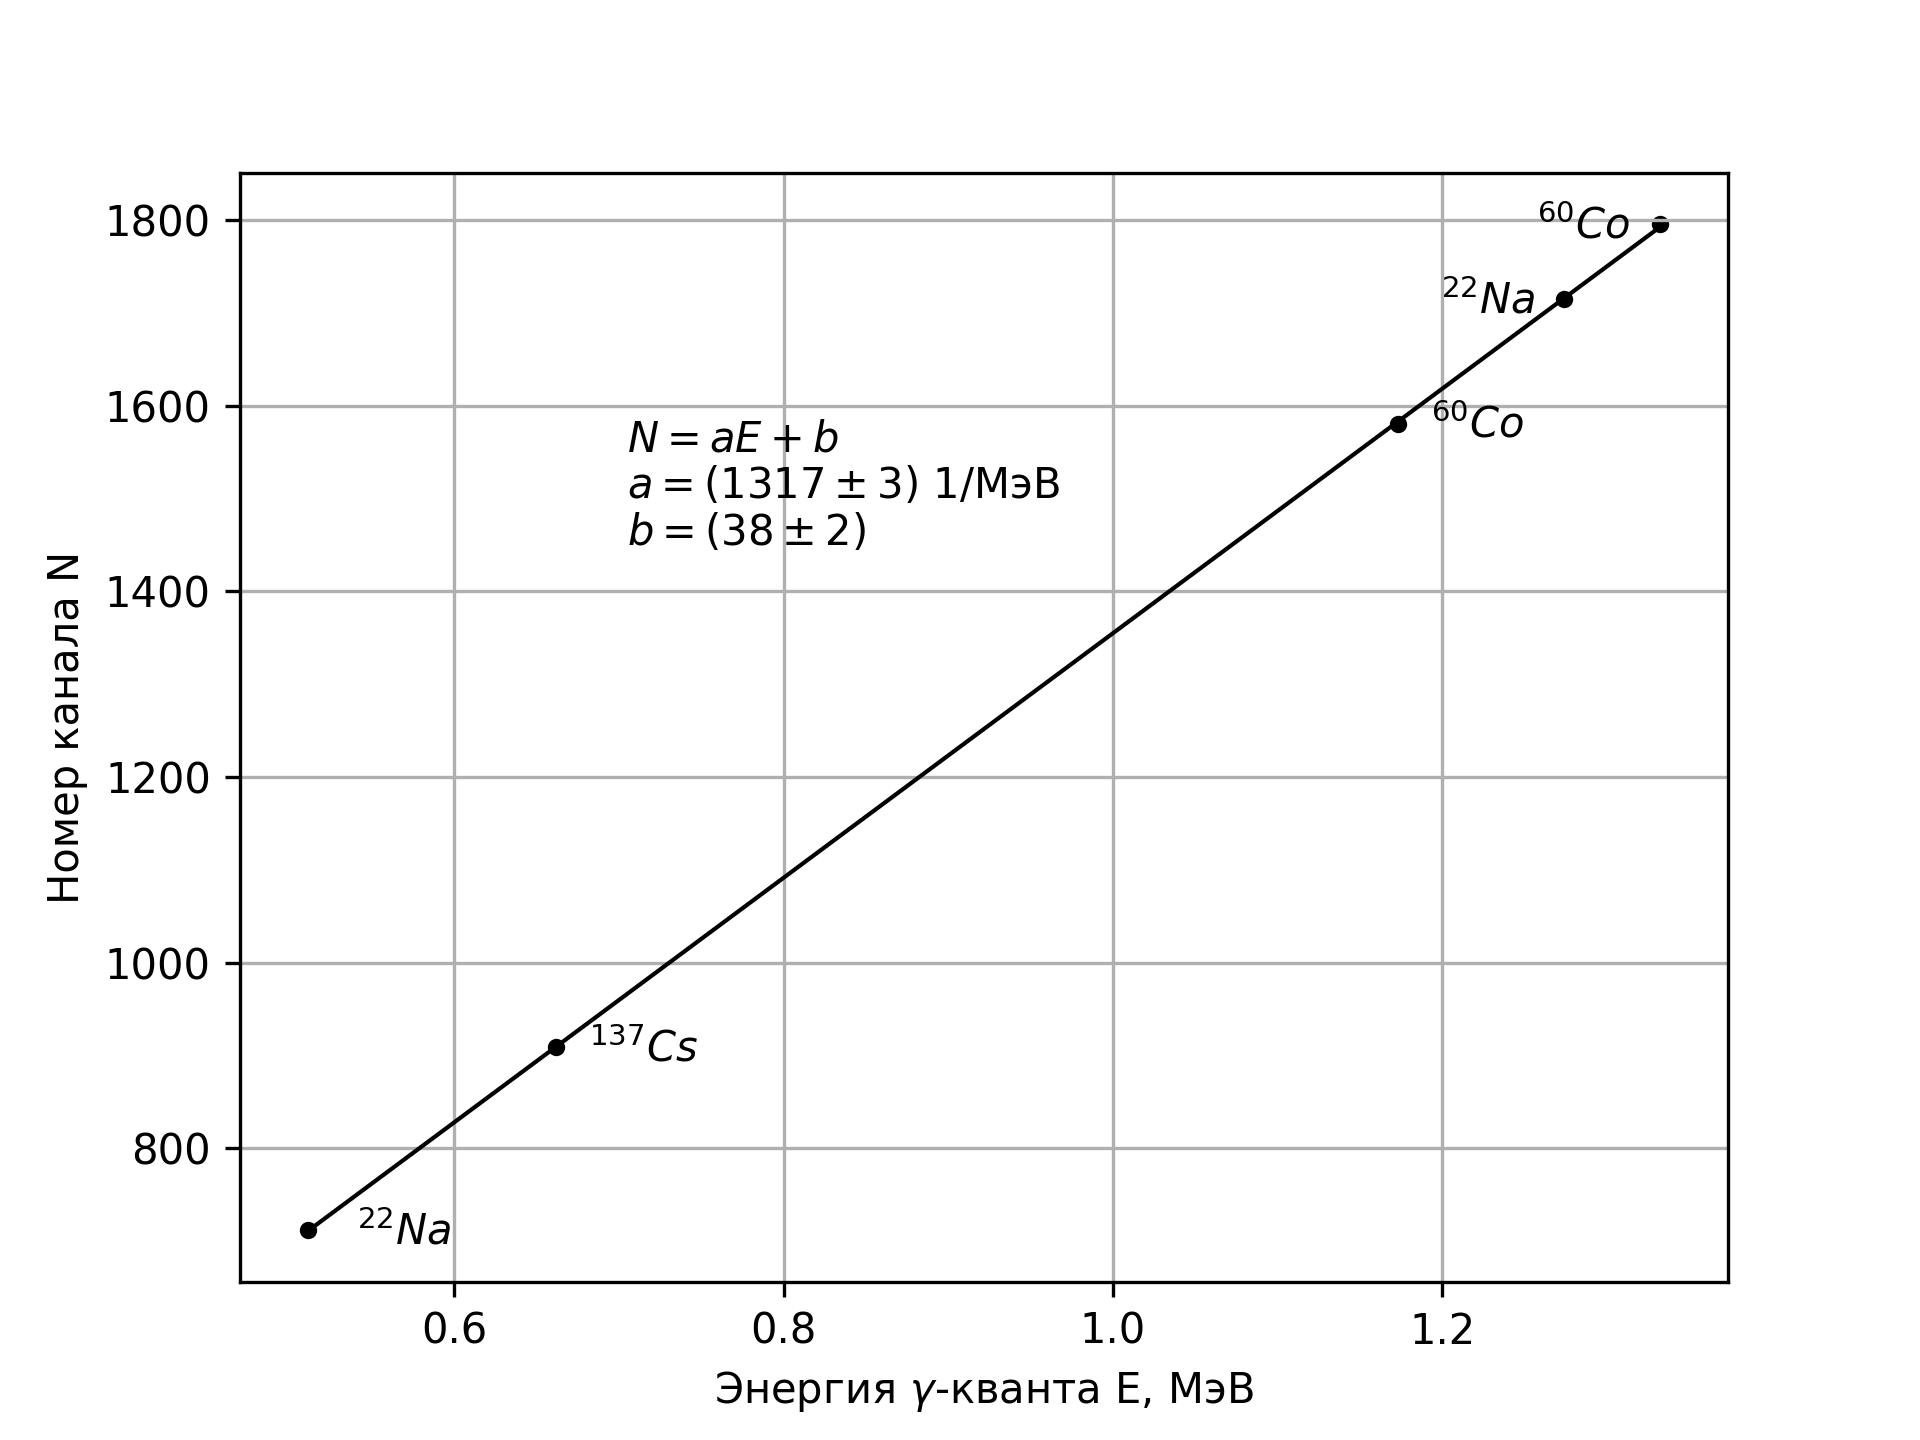
\includegraphics[width=.7\textwidth]{../images/555-cal}
\caption{Калибровочная прямая}
\end{figure}

\subsection{$^{152}\text{Eu}$}

\begin{figure}[H]
\centering
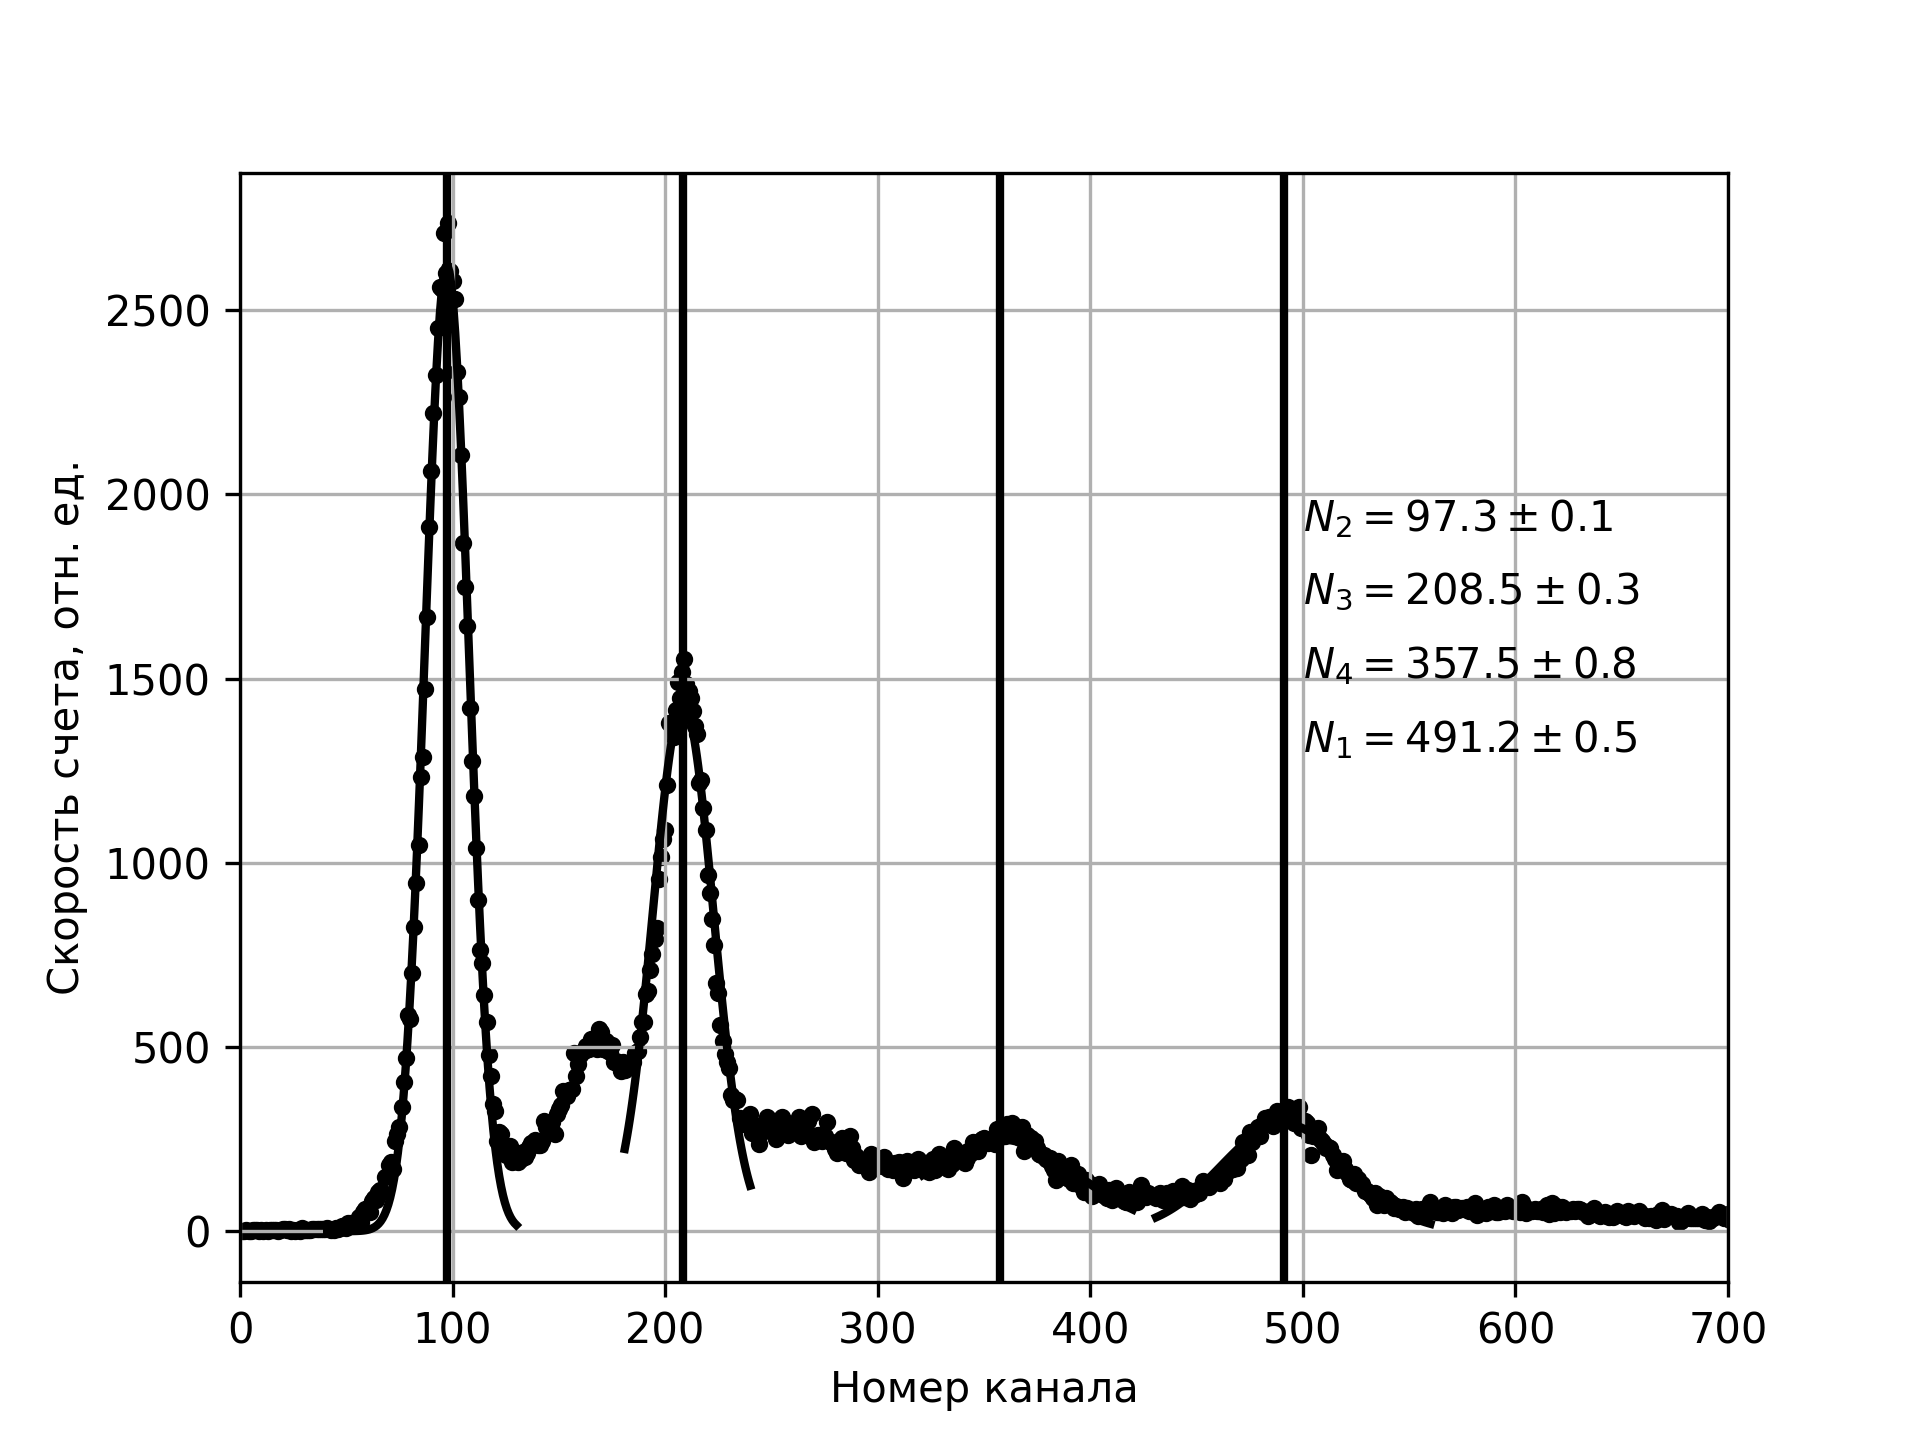
\includegraphics[width=.7\textwidth]{../images/555-eu152}
\caption{Спектр излучения $^{152}\text{Eu}$}
\end{figure}

В спектре европия-152 удалось выделить четыре пика.

\subsection{$^{241}\text{Am}$}

\begin{figure}[H]
\centering
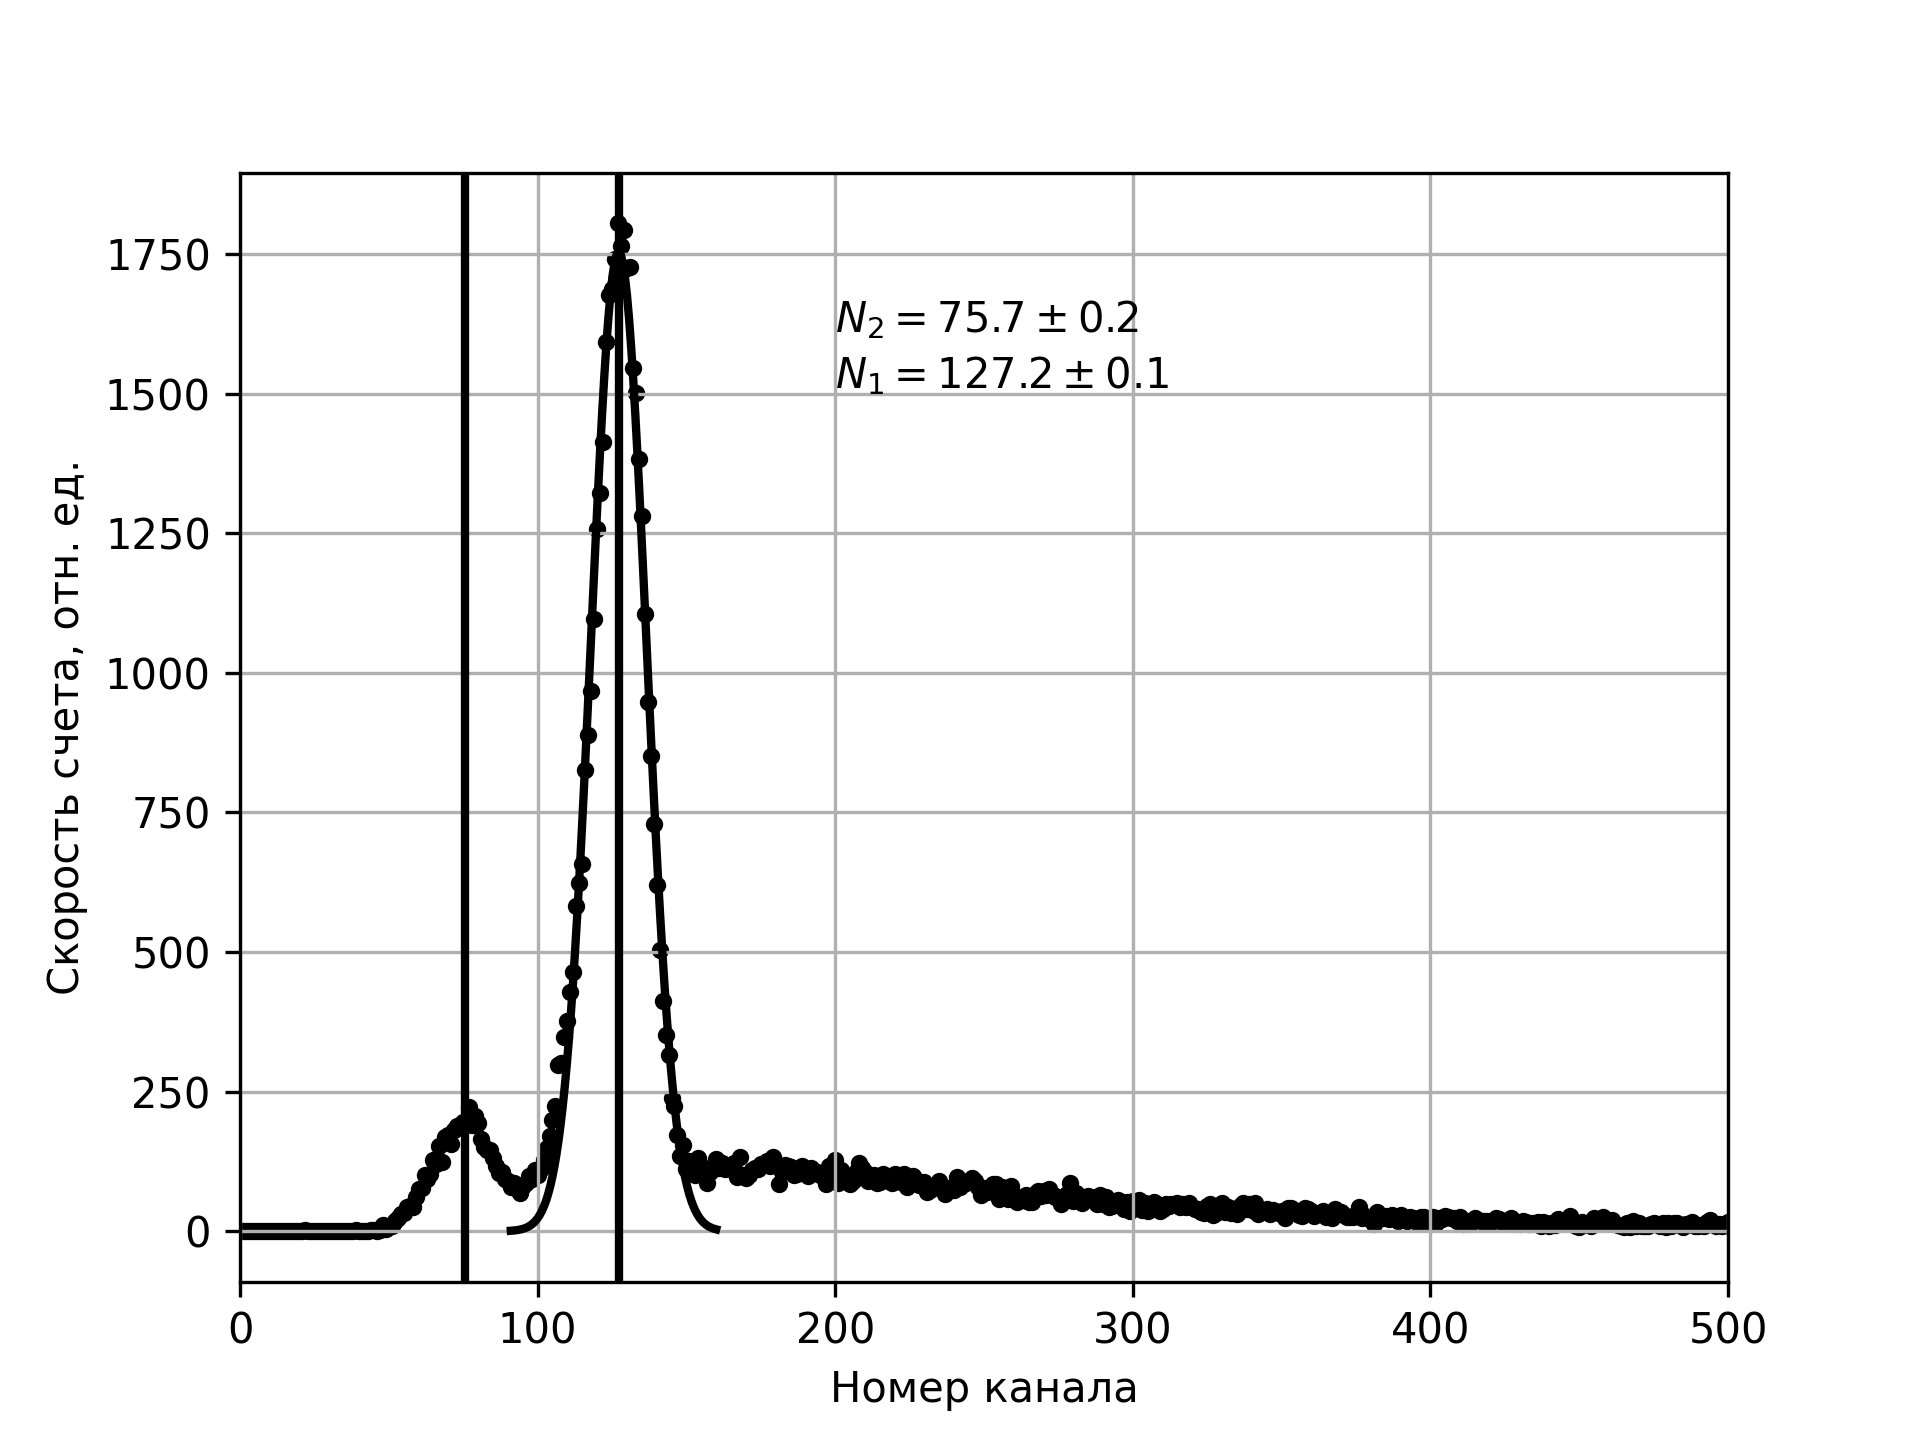
\includegraphics[width=.7\textwidth]{../images/555-am241}
\caption{Спектр излучения $^{241}\text{Am}$}
\end{figure}

В спектре америция-241 удалось выделить два пика.

\subsection{Сводная таблица}

\begin{table}[H]
\centering
\begin{tabular}{|c|c|c|c|c|c|}
\hline
Источник & N & $\Delta$N & E, МэВ & $\Delta$E, МэВ & R \\ \hline
$^{60}\text{Co}$       & 1580  & 127 & 1.17 &0.10& 0.082\\ \hline
$^{60}\text{Co}$       & 1795  & 114 & 1.33 &0.09& 0.065\\ \hline
$^{22}\text{Na}$       & 1715  & 143 & 1.27 &0.11& 0.085\\ \hline
$^{22}\text{Na}$       & 712 & 73 & 0.511 &0.05&0.11\\ \hline
$^{137}\text{Cs}$       & 909 & 75 & 0.661 &0.06&0.086\\ \hline
$^{152}\text{Eu}$       & 491 & 70 & 0.344 &0.05&0.15\\ \hline
$^{152}\text{Eu}$       & 97 & 24 & 0.045 &0.02&0.41\\ \hline
$^{152}\text{Eu}$       & 208 & 34 & 0.129 &0.03&0.20\\ \hline
$^{152}\text{Eu}$       & 357 & 87 & 0.243 &0.07&0.27\\ \hline
$^{241}\text{Am}$       & 127 & 22& 0.068 &0.02&0.24\\ \hline
$^{241}\text{Am}$       & 75 & 26 & 0.029 &0.02&0.68\\ \hline
\end{tabular}
\end{table}

Спектры европия-152 и америция-241 можно найти в интернете и сравнить значения энергий фотопиков. У европия-152 действительно существуют пики на 40 кэВ, 344.2785 кэВ, 244.6975 кэВ, 121.7817 кэВ (https://www.gammaspectacular.com/blue/eu152-spectrum). У америция-241 существуют хорошо известные пики на 59.6 кэВ и 26.3 кэВ (https://www.gammaspectacular.com/blue/am241-spectrum).

\subsection{Энергетическое разрешение}

Проверим зависиость $R=\frac{C}{\sqrt{E}}$. Для этого отложим экспериментальные точки в осях $R^2$ от $1/E$.

\begin{figure}[H]
\centering
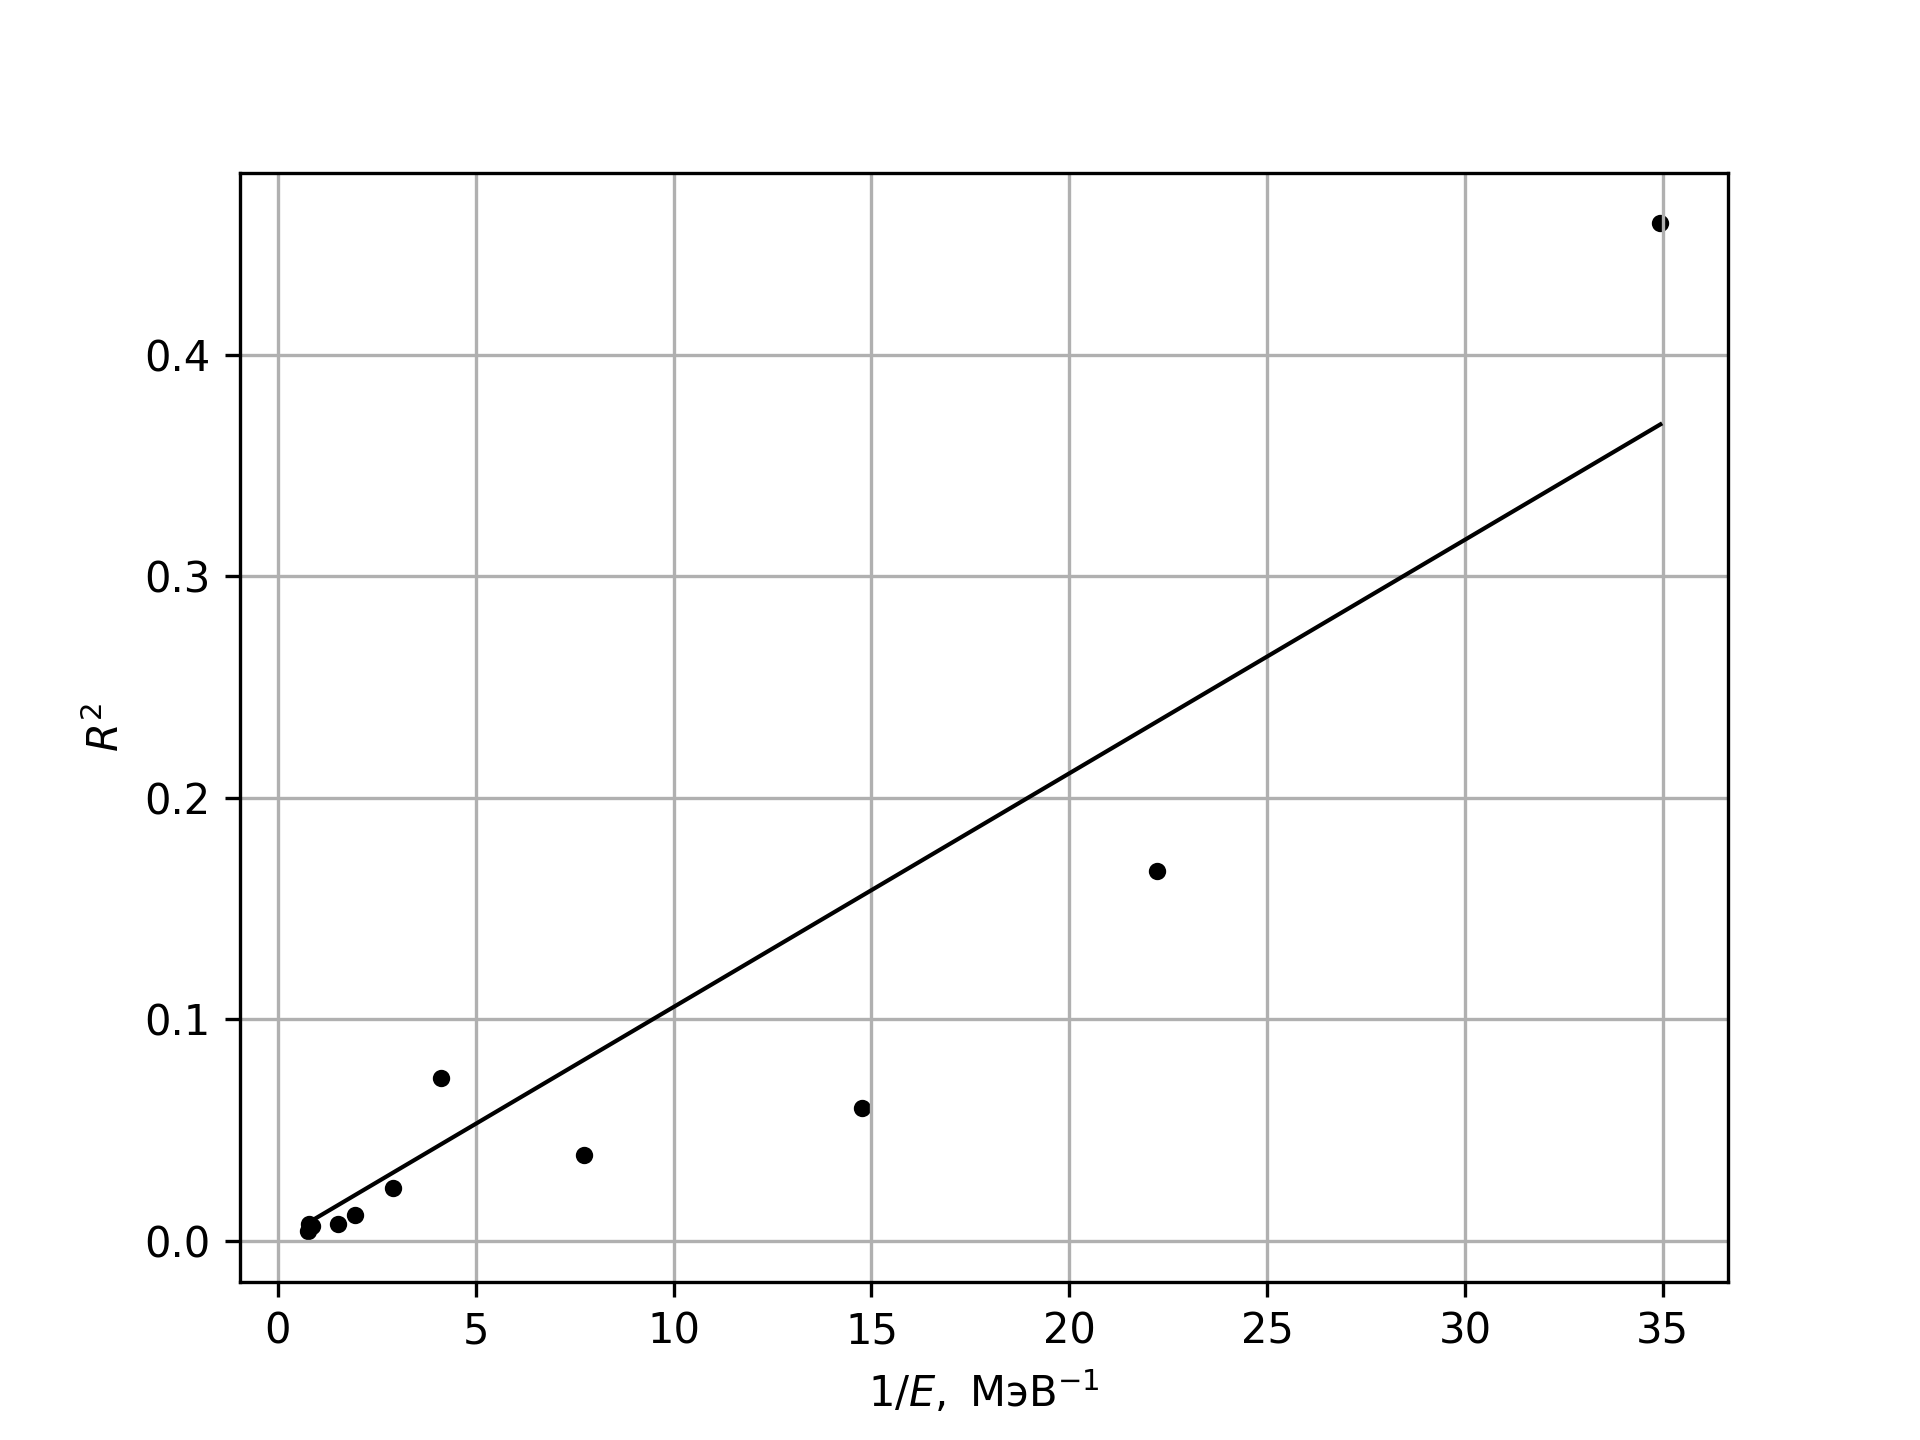
\includegraphics[width=.7\textwidth]{../images/555-R}
\caption{График зависимости $R^2=1/E$}
\end{figure}

Проведем через точки прямую вида $y=kx$. Получим, что постоянная $C\approx(0.011\pm0.01)\ \text{МэВ}^{-1/2}$

\subsection{Наблюдения на осциллографе}

\begin{figure}[H]
\centering
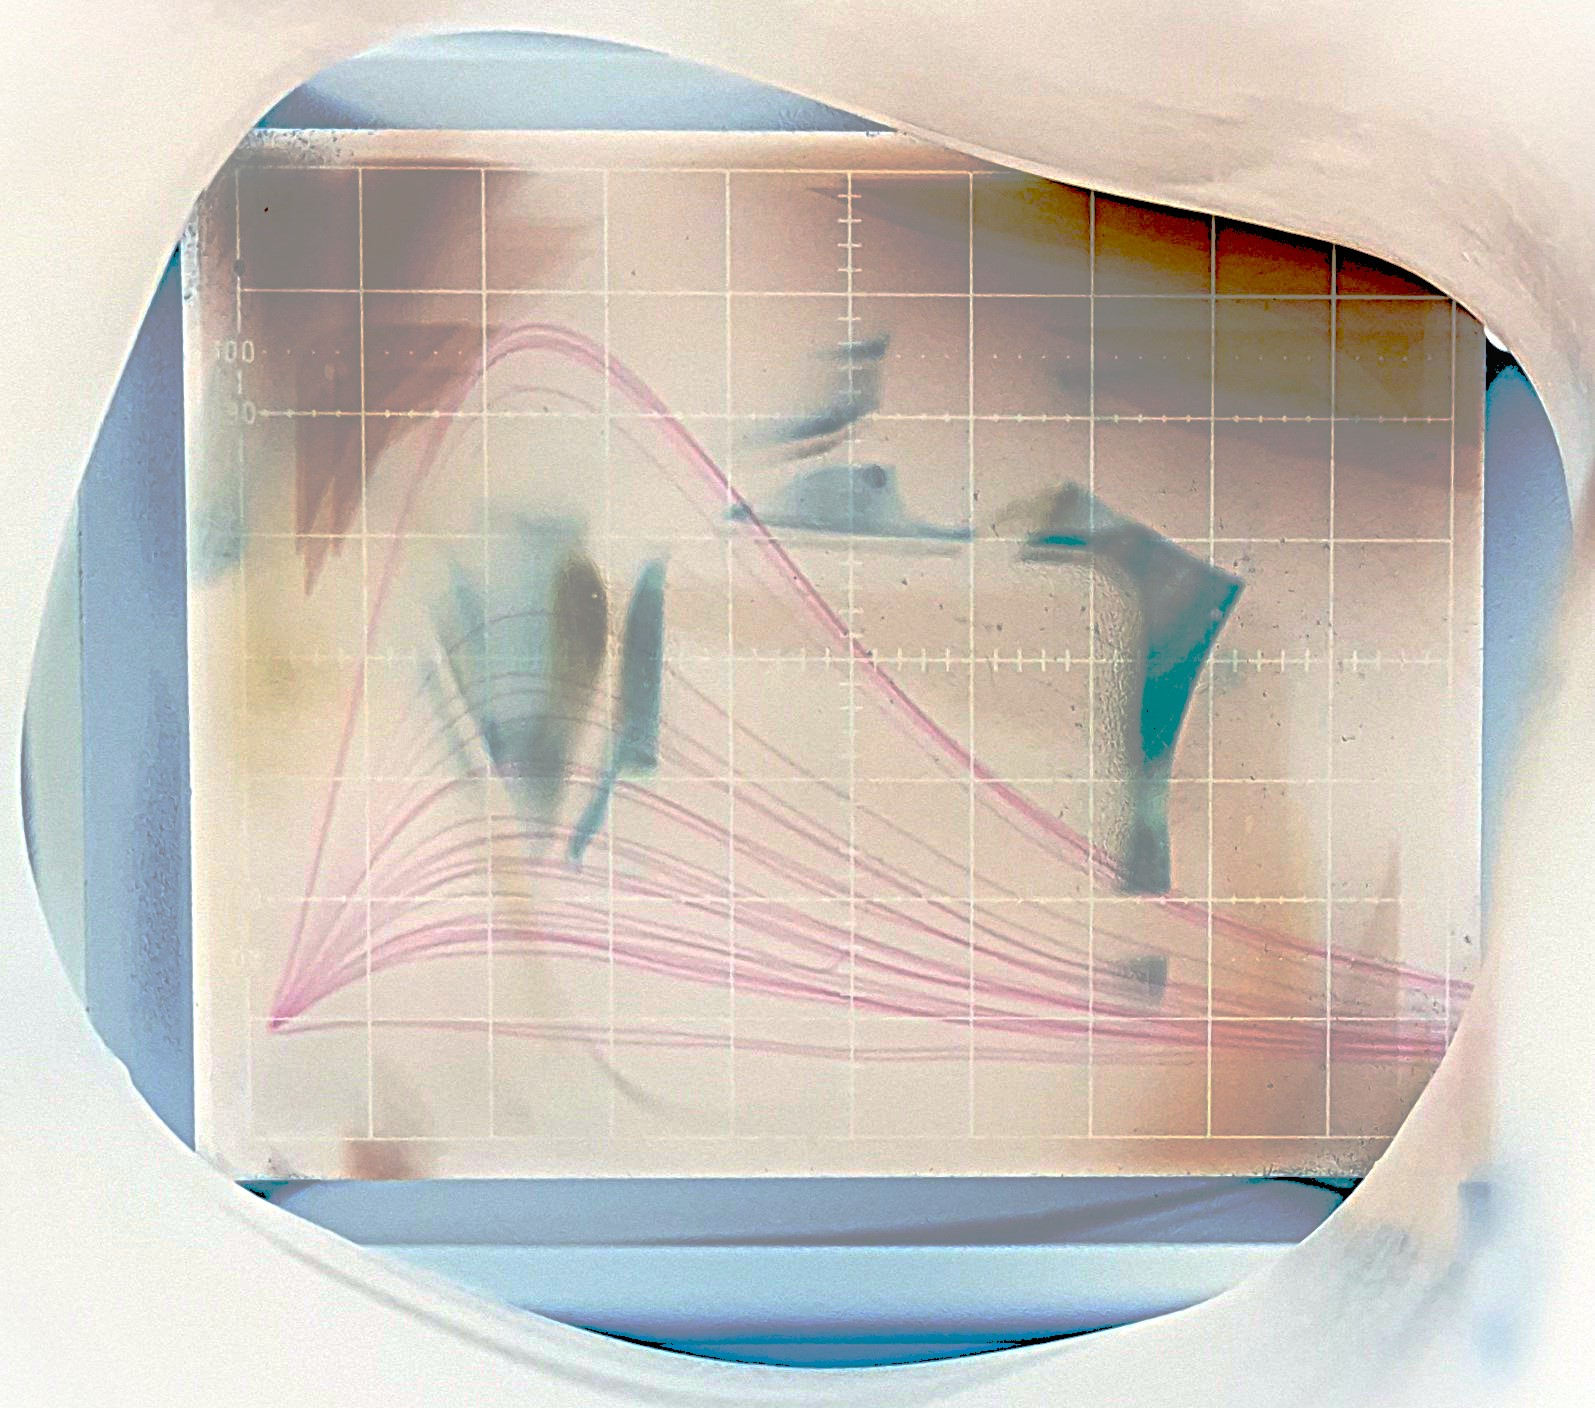
\includegraphics[width=.7\textwidth]{../images/555-PMT}
\caption{График зависимости $R^2=1/E$}
\end{figure}

\subsection{Пик обратного рассеяния}

Данный пик хорошо различим на спектрах только двух образцов: цезия и кобальта (если из спектров вычесть фон).

\begin{figure}[H]
\centering
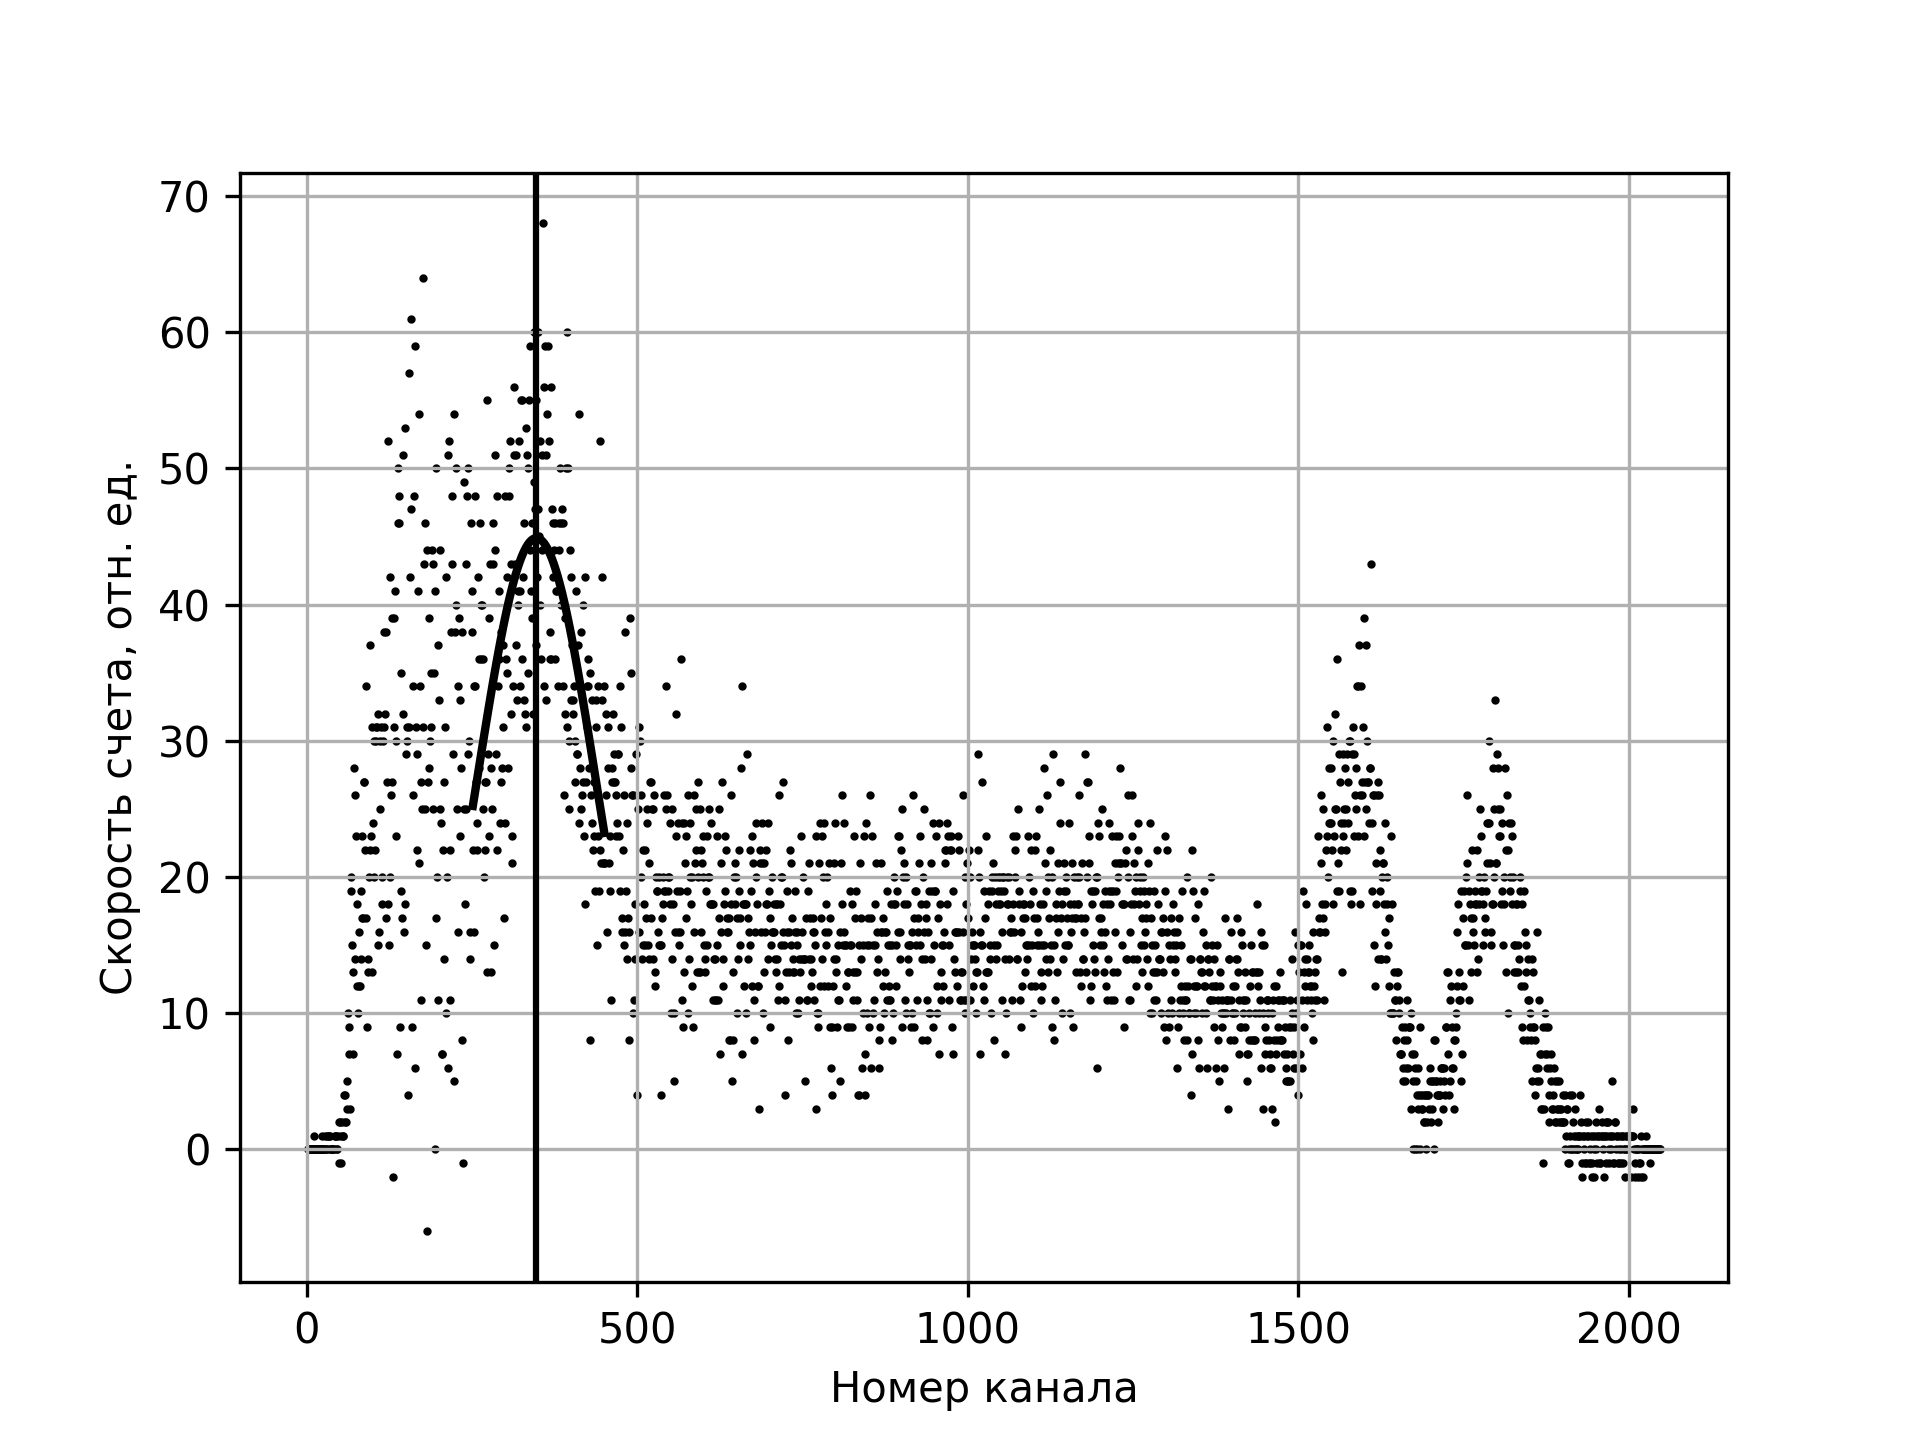
\includegraphics[width=.7\textwidth]{../images/555-co60bs}
\caption{Спектр излучения $^{60}\text{Co}$ без фона}
\end{figure}

\begin{figure}[H]
\centering
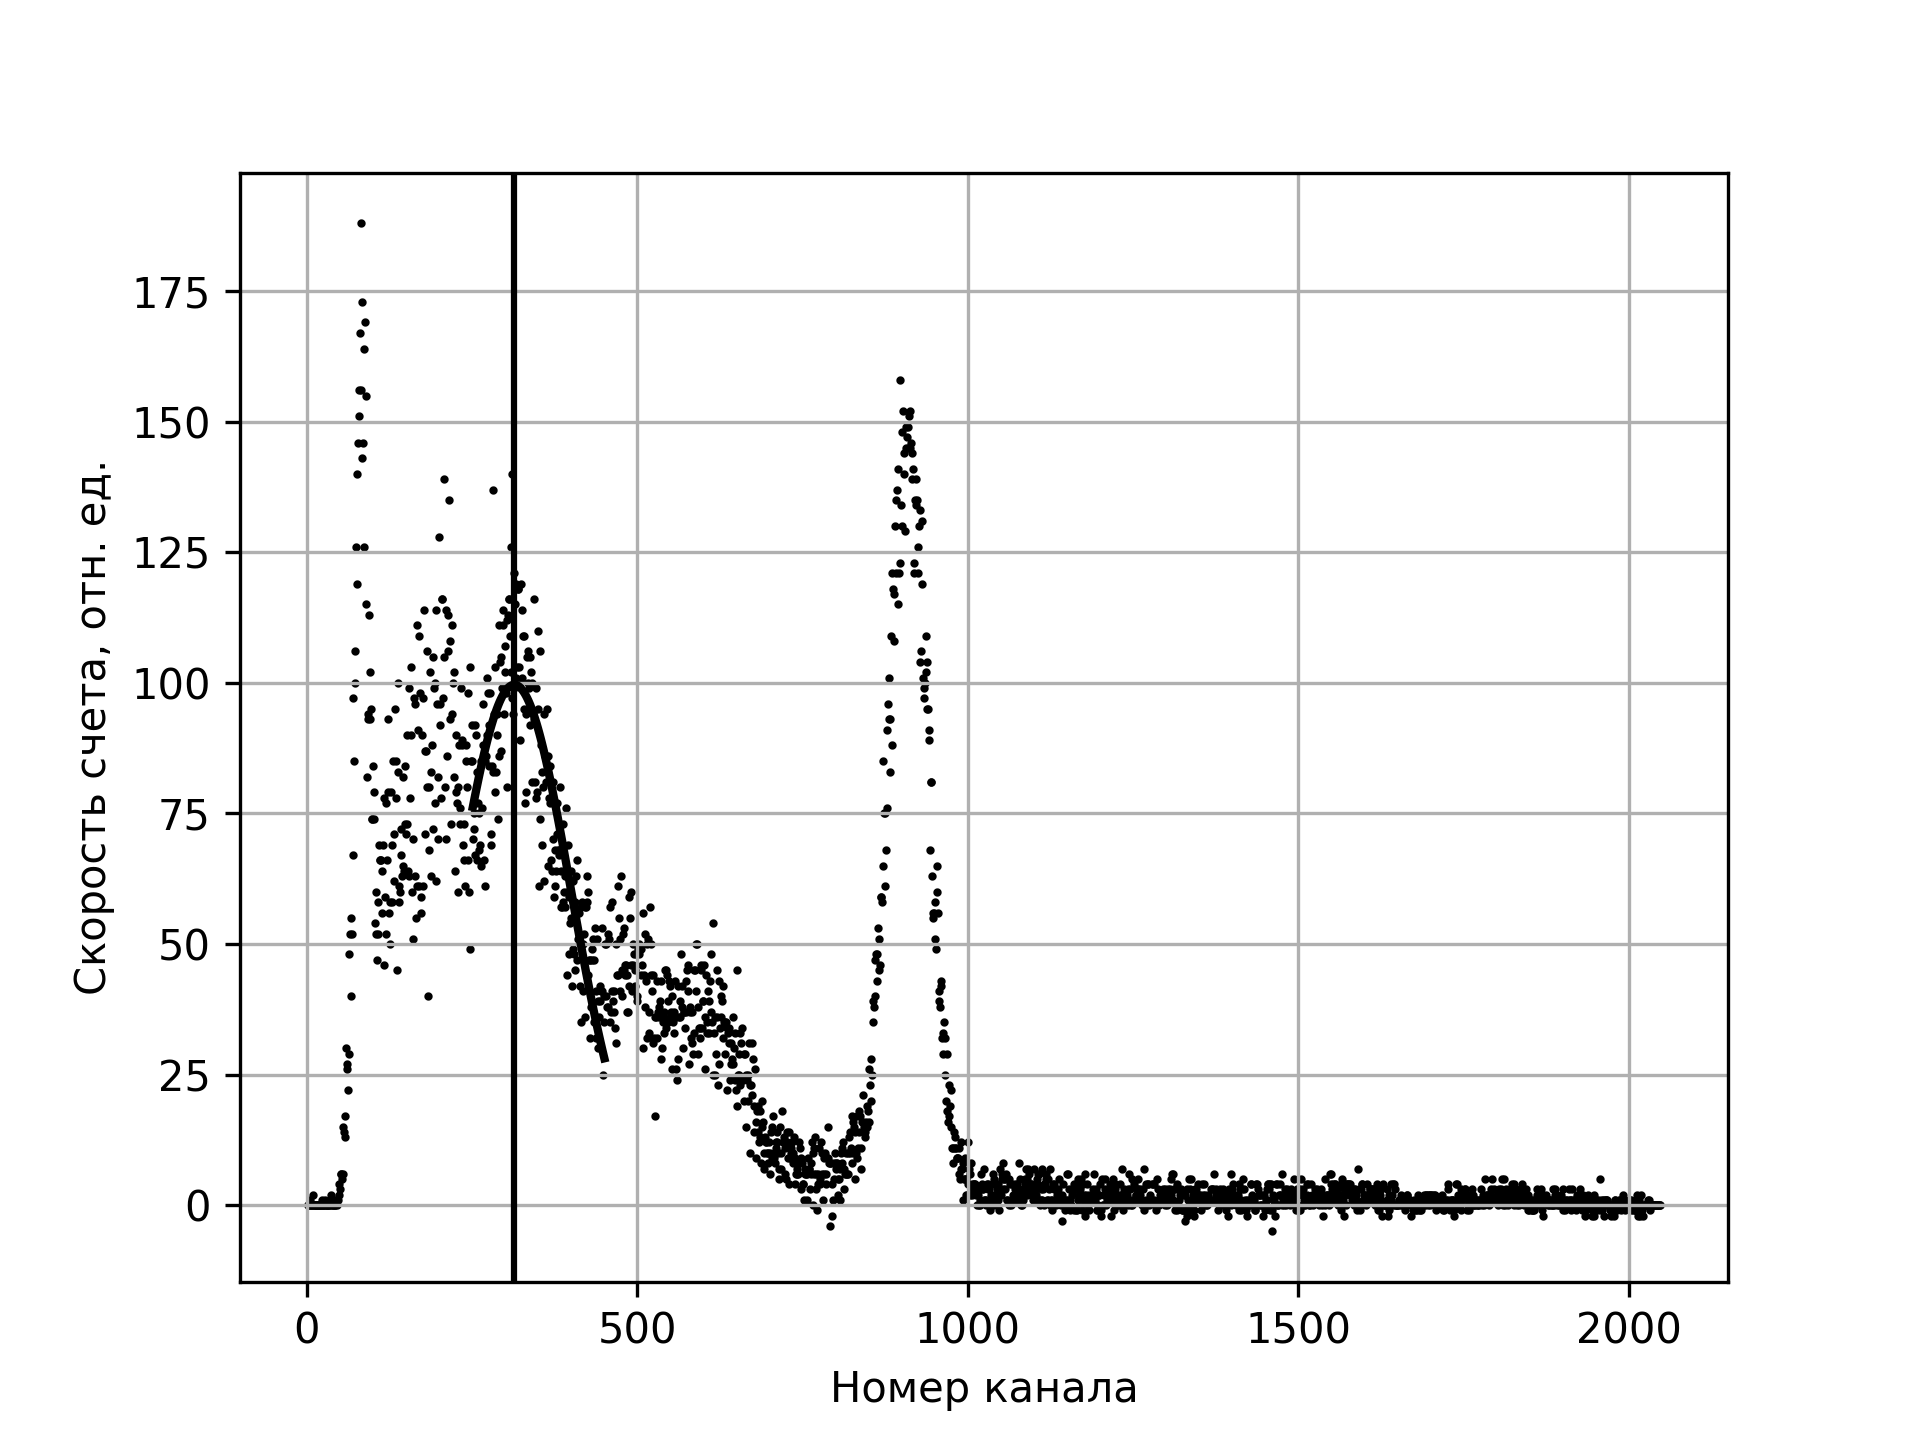
\includegraphics[width=.7\textwidth]{../images/555-cs137bs}
\caption{Спектр излучения $^{137}\text{Cs}$ без фона}
\end{figure}

Получим энергии 0.235 МэВ и 0.210 МэВ соответственно.

\end{document}